\documentclass[a4paper,11pt]{book}
%\documentclass[a4paper,twoside,11pt,titlepage]{book}
\usepackage{listings}
\usepackage[utf8]{inputenc}
\usepackage[spanish]{babel}
\usepackage[T1]{fontenc}

\usepackage[usenames, dvipsnames]{color}
\usepackage{titlesec}
\usepackage{titling}
\usepackage{indentfirst}
\usepackage{float}
\usepackage{setspace} 
\usepackage{tabularx}
\usepackage[labelfont=bf,textfont=bf]{caption}
\usepackage[toc,page]{appendix}
\usepackage{verbatim} % comentarios
\usepackage{multicol}
\usepackage{multirow}
\usepackage{subcaption}




% Definir los márgenes
%\usepackage[a4paper, left = 1.18in, right = 0.79in, top = 1.18in, bottom = 0.79in]{geometry}

% \usepackage[style=list, number=none]{glossary} %
%\usepackage{titlesec}
%\usepackage{pailatino}

\decimalpoint
\usepackage{dcolumn}
\newcolumntype{.}{D{.}{\esperiod}{-1}}
\makeatletter
\addto\shorthandsspanish{\let\esperiod\es@period@code}
\makeatother

%\usepackage[chapter]{algorithm}
\RequirePackage{verbatim}
%\RequirePackage[Glenn]{fncychap}
\usepackage{fancyhdr}
\usepackage{graphicx}
\usepackage{afterpage}

\usepackage{longtable}

\usepackage{colortbl, longtable}
\usepackage[table,xcdraw]{xcolor}

\usepackage[pdfborder={000}]{hyperref} %referencia

\usepackage{rotating}

\newcommand\tab[1][1cm]{\hspace*{#1}}

% ********************************************************************
% Re-usable information
% ********************************************************************
\newcommand{\myTitle}{Integración de Información Geográfica en la Web Semántica\xspace}
\newcommand{\myDegree}{Máster en Ingeniería Informática\xspace}
\newcommand{\myName}{Gema Correa Fernández\xspace}
\newcommand{\myOtherProf}{José Samos Jimenéz\xspace}
%\newcommand{\mySupervisor}{Put name here\xspace}
\newcommand{\myFaculty}{Escuela Técnica Superior de Ingenierías Informática y de
Telecomunicación\xspace}
\newcommand{\myFacultyShort}{E.T.S. de Ingenierías Informática y de
Telecomunicación\xspace}
\newcommand{\myDepartment}{Departamento de Lenguajes y Sistemas Informáticos\xspace}
\newcommand{\myUni}{\protect{Universidad de Granada}\xspace}
\newcommand{\myLocation}{Granada\xspace}
\newcommand{\myTime}{\today\xspace}
\newcommand{\myVersion}{Version 0.1\xspace}

\hypersetup{
pdfauthor = {\myName (gecorrea@correo.ugr.es)},
pdftitle = {\myTitle},
pdfsubject = {Sistemas de Información Geográfica},
pdfkeywords = {palabra_clave1, palabra_clave2, palabra_clave3, ...},
pdfcreator = {LaTeX con el paquete ....},
pdfproducer = {pdflatex}
}

%\hyphenation{}


%\usepackage{doxygen/doxygen}
%\usepackage{pdfpages}
\usepackage{url}
\usepackage{colortbl,longtable}
\usepackage[stable]{footmisc}
%\usepackage{index}

%\makeindex
%\usepackage[style=long, cols=2,border=plain,toc=true,number=none]{glossary}
% \makeglossary

% Definición de comandos que me son tiles:
%\renewcommand{\indexname}{Índice alfabético}
%\renewcommand{\glossaryname}{Glosario}

\pagestyle{fancy}
\fancyhf{}
\fancyhead[LO]{\leftmark}
\fancyhead[RE]{\rightmark}
\fancyhead[RO,LE]{\textbf{\thepage}}
\renewcommand{\chaptermark}[1]{\markboth{\textbf{#1}}{}}
\renewcommand{\sectionmark}[1]{\markright{\textbf{\thesection. #1}}}

\setlength{\headheight}{1.5\headheight}

\newcommand{\HRule}{\rule{\linewidth}{0.5mm}}
%Definimos los tipos teorema, ejemplo y definición podremos usar estos tipos
%simplemente poniendo \begin{teorema} \end{teorema} ...
\newtheorem{teorema}{Teorema}[chapter]
\newtheorem{ejemplo}{Ejemplo}[chapter]
\newtheorem{definicion}{Definición}[chapter]

\definecolor{gray97}{gray}{.97}
\definecolor{gray75}{gray}{.75}
\definecolor{gray45}{gray}{.45}
\definecolor{gray30}{gray}{.94}
\definecolor{airforceblue}{rgb}{0.36, 0.54, 0.66}
\definecolor{arsenic}{rgb}{0.23, 0.27, 0.29}
\definecolor{blue(munsell)}{rgb}{0.0, 0.5, 0.69}
\definecolor{bondiblue}{rgb}{0.0, 0.58, 0.71}
\definecolor{bluegray}{rgb}{0.4, 0.6, 0.8}
\definecolor{cadet}{rgb}{0.23, 0.41, 0.67}
\definecolor{britishracinggreen}{rgb}{0.0, 0.26, 0.15}
\definecolor{oldrose}{rgb}{0.75, 0.5, 0.51}
\definecolor{oldmauve}{rgb}{0.4, 0.19, 0.28}
\definecolor{pastelgray}{rgb}{0.81, 0.81, 0.77}
\definecolor{gray15}{gray}{.30}
\definecolor{gray(x11gray)}{rgb}{0.97, 0.97, 0.97}
\definecolor{mygray}{rgb}{0.5,0.5,0.5}
\definecolor{codegreen}{rgb}{0,0.6,0}
\definecolor{codegray}{rgb}{0.5,0.5,0.5}
\definecolor{codepurple}{rgb}{0.58,0,0.82}
\definecolor{backcolour}{rgb}{0.95,0.95,0.92}

\usepackage{natbib}


\usepackage{comment}

\begin{comment}
	\lstset{ frame=Ltb,
	framerule=0.5pt,
	aboveskip=0.5cm,
	framextopmargin=3pt,
	framexbottommargin=3pt,
	framexleftmargin=0.1cm,
	framesep=0pt,
	rulesep=.4pt,
	backgroundcolor=\color{gray97},
	rulesepcolor=\color{black},
	%
	stringstyle=\ttfamily,
	showstringspaces = false,
	basicstyle=\scriptsize\ttfamily,
	commentstyle=\color{gray45},
	keywordstyle=\bfseries,
	%
	numbers=left,
	numbersep=6pt,
	numberstyle=\tiny,
	numberfirstline = false,
	breaklines=true,
	}
\end{comment}

 \usepackage{hvfloat}
 
% minimizar fragmentado de listados
\lstnewenvironment{listing}[1][]
   {\lstset{#1}\pagebreak[0]}{\pagebreak[0]}

\lstdefinestyle{CodigoC}
   {
	basicstyle=\scriptsize,
	frame=single,
	language=C,
	numbers=left
   }
\lstdefinestyle{CodigoC++}
   {
	basicstyle=\small,
	frame=single,
	backgroundcolor=\color{gray30},
	language=C++,
	numbers=left
   }

 
\lstdefinestyle{Consola}
   {basicstyle=\scriptsize\bf\ttfamily,
    backgroundcolor=\color{gray30},
    frame=single,
    numbers=none
   }
  
\lstdefinestyle{mystyle}{
	backgroundcolor=\color{gray(x11gray)},   
	commentstyle=\color{codegreen},
	%keywordstyle=\color{magenta},
	numberstyle=\tiny\color{codegray},
	stringstyle=\color{codepurple},
	basicstyle=\small\sffamily,
	breakatwhitespace=false,         
	breaklines=true,                 
	captionpos=b,                    
	keepspaces=true,                 
	numbers=left,                    
	numbersep=5pt,                  
	showspaces=false,                
	showstringspaces=false,
	showtabs=false,                  
	tabsize=2,
	morekeywords={*,+,<-, =, function}  
}

%"mystyle" code listing set
\lstset{style=mystyle}


\newcommand{\bigrule}{\titlerule[0.5mm]}


%Para conseguir que en las páginas en blanco no ponga cabecerass
\makeatletter
\def\clearpage{%
  \ifvmode
    \ifnum \@dbltopnum =\m@ne
      \ifdim \pagetotal <\topskip
        \hbox{}
      \fi
    \fi
  \fi
  \newpage
  \thispagestyle{empty}
  \write\m@ne{}
  \vbox{}
  \penalty -\@Mi
}
\makeatother

\usepackage{pdfpages}

\begin{document}

\begin{titlepage}
 
 
\newlength{\centeroffset}
\setlength{\centeroffset}{-0.5\oddsidemargin}
\addtolength{\centeroffset}{0.5\evensidemargin}
\thispagestyle{empty}

\noindent\hspace*{\centeroffset}\begin{minipage}{\textwidth}

\centering
\includegraphics[width=0.9\textwidth]{imagenes/logo_ugr.jpg}\\[1.4cm]

\textsc{ \Large TRABAJO FIN DE MÁSTER\\[0.2cm]}
\textsc{ MÁSTER UNIVERSITARIO EN INGENIERÍA INFORMÁTICA}\\[1cm]
% Upper part of the page
% 
% Title
{\huge\bfseries Integración de Información Geográfica en la Web Semántica\\
}
\noindent\rule[-1ex]{\textwidth}{3pt}\\[3.5ex]
{\Large\bfseries SUBTÍTULO}
\end{minipage}

\vspace{2cm}
\noindent\hspace*{\centeroffset}\begin{minipage}{\textwidth}
\centering

\textbf{Autora}\\ {Gema Correa Fernández}\\[2.5ex]
\textbf{Director}\\
{José Samos Jiménez}\\[2cm]
\includegraphics[width=0.3\textwidth]{imagenes/etsiit_logo.png}\\[0.1cm]
\textsc{Escuela Técnica Superior de Ingenierías Informática \\y de Telecomunicación}\\
\textsc{---}\\
Granada, \today
\end{minipage}
%\addtolength{\textwidth}{\centeroffset}
%\vspace{\stretch{2}}
\end{titlepage}



\chapter*{}
\thispagestyle{empty}
%\cleardoublepage

%\thispagestyle{empty}

\begin{titlepage}
 
 
\setlength{\centeroffset}{-0.5\oddsidemargin}
\addtolength{\centeroffset}{0.5\evensidemargin}
\thispagestyle{empty}

\noindent\hspace*{\centeroffset}\begin{minipage}{\textwidth}

\centering
%\includegraphics[width=0.9\textwidth]{imagenes/logo_ugr.jpg}\\[1.4cm]

%\textsc{ \Large PROYECTO FIN DE CARRERA\\[0.2cm]}
%\textsc{ INGENIERÍA EN INFORMÁTICA}\\[1cm]
% Upper part of the page
% 

\vspace{0.15cm}

%si el proyecto tiene logo poner aquí
\includegraphics[scale=0.25]{imagenes/ugr_logo.jpg} 
 %\vspace{0.95cm}
 
\begin{center}
    Gema Correa Fernández
\end{center}

\vspace{0.5in}
 
% Title
{\LARGE\bfseries Integración de Información Geográfica en la Web Semántica\\
}
\noindent\rule[-1ex]{\textwidth}{0.5pt}\\[3.5ex]
{\Large\bfseries SUBTÍTULO\\[4cm]}
\end{minipage}

\vspace{4.75cm}
\noindent\hspace*{\centeroffset}\begin{minipage}{\textwidth}
\centering

%\textbf{Autor}\\ {Gema Correa Fernández}\\[2.5ex]
%\textbf{Directores}\\
%{José Samos Jiménez}\\[2cm]
%\includegraphics[width=0.15\textwidth]{imagenes/tstc.png}\\[0.1cm]
%\textsc{Departamento de Teoría de la Señal, Telemática y Comunicaciones}\\
%\textsc{---}\\

\begin{flushright}
    Trabajo de Fin de Máster para la integración de Información Geográfica \\ en la Web Semántica del Departamento de Lenguajes y Sistemas \\ Informáticos de la Escuela Técnica Superior de Ingenierías \\ Informáticas y de Telecomunicaciones de la UGR \\
    
    \vspace{0.2in}
    
    Director: José Samos Jiménez
\end{flushright}

\vspace{4cm}
Septiembre de 2019
\end{minipage}
%\addtolength{\textwidth}{\centeroffset}
\vspace{\stretch{2}}

 
\end{titlepage}






\cleardoublepage
\thispagestyle{empty}

\begin{center} 
	\large{\textbf{Integración de Información Geográfica en la Web Semántica:\\ Ontología GEOARES}}\\
	\vspace{0.25in}
	Gema Correa Fernández
\end{center}


\section*{Resumen}

% Este trabajo tiene como objetivo el análisis de Información Geográfica mediante el uso de las herramientas QGIS y R, herramientas de software libre de amplia difusión. En particular, está centrado en el estudio del Modelo Digital del Terreno. Para entender el ámbito, se contextualizan y desarrollan los conceptos necesarios del área de los Sistemas de Información Geográfica. El Modelo Digital del Terreno es un modelo de datos que permite la realización de análisis sofisticados; estos análisis se pueden realizar tanto en QGIS como en R. En el trabajo se profundizan y se estudian los análisis considerados más relevantes para este ámbito con ambas herramientas, realizando una comparación y evaluación de ambas. A modo de ejemplo se realiza el análisis para la parte occidental de la Vega de Granada. Los datos utilizados y las funciones desarrolladas mediante paquetes existentes de R, se han estructurado en forma de un nuevo paquete. Por el enfoque que se realiza, este trabajo puede resultar de utilidad para aquellas personas que se adentran en este tema.

Este trabajo tiene como objetivo estudiar las herramientas de la Web Semántica que se pueden utilizar para representar e integrar Información Geográfica. En particular, está centrado en valorar las posibles herramientas y tecnologías que ofrece la Web Semántica mediante el desarrollo de una prueba de concepto con Información Geográfica procedente de la provincia de Granada, a través de la creación de la ontología GEOARES. Para entender el ámbito de aplicación, se contextualizan y desarrollan los conceptos necesarios en el ámbito de los Sistemas de Información Geográfica y Web Semántica, esta última área ofrece mecanismos muy útiles para la representación de estándares e incorporación de información geoespacial. Gracias a la capa semántica que ofrecen los Sistemas de Información Geográfica es posible agregar conocimiento de dominio sobre la estructura de los datos de la Web Semántica y consultar dicha información haciendo uso de los estándares definidos. Por el enfoque que se realiza, este trabajo puede resultar de utilidad para aquellas personas que quieren seguir aprendiendo sobre los Sistemas de Información Geográfica en un ámbito distinto y quieren adentrarse en la Web Semántica.



\vspace{0.25in}

{\bf Palabras-clave:} Sistemas de Información Geográfica, SIG, Web actual, Web Semántica, OWL, RDF, SPARQL, GeoSPARQL, Shapefile, QGIS, R,  Protegé, GraphBD.

\cleardoublepage


\thispagestyle{empty}


\begin{center} 
	\large{\textbf{Integration of Geographic Information in the Semantic Web:\\ GEOARES Ontology}}\\
	\vspace{0.25in}
	Gema Correa Fernández
\end{center}

\section*{Abstract} 

The purpose of this project is study the tools of the Semantic Web that can be used to represent and integrate Geographic Information. In particular, it is focused on assessing the possible tools and technologies offered by the Semantic Web by developing a proof of concept with Geographic Information from the province of Granada, through the creation of the GEOARES ontology. To understand the scope, the necessary concepts are contextualized and developed in the field of Geographic Information Systems and Semantic Web, the latter area offers very useful mechanisms for the representation of standards and incorporation of geospatial information. Thanks to the semantic layer offered by the Geographic Information Systems it is possible to add domain knowledge about the structure of the data of the Semantic Web and consult this information using the defined standards. Due to the approach carried out, this work can be useful for those who want to continue learning about Geographic Information Systems in a different area and want to enter the Semantic Web.


\vspace{0.25in}

{\bf Key-words:} Geographic Information Systems, GIS, Current Web, Semantic Web, OWL, RDF, SPARQL, GeoSPARQL, Shapefile, QGIS, R, Protegé, GraphBD.

\chapter*{}
\thispagestyle{empty}

\noindent\rule[-1ex]{\textwidth}{2pt}\\[4.5ex]

Yo, \textbf{Gema Correa Fernández}, alumna del Máster Universitario de Ingeniería Informática de la \textbf{Escuela Técnica Superior de Ingenierías Informática y de Telecomunicación de la Universidad de Granada}, con DNI 75572158-T, autorizo la ubicación de la siguiente copia de mi Trabajo Fin de Máster en la biblioteca del centro para que pueda ser consultada por las personas que lo deseen.\newline

Asimismo, el código fuente del proyecto y esta documentación pueden consultarse en la dirección \url{https://github.com/Gecofer/TFM} una vez defendido el TFM, para que aquellos que lo deseen puedan conocer el proyecto.

\vspace{5cm}

\noindent Fdo: Gema Correa Fernández

\vspace{2cm}

\begin{flushright}
Granada a \today
\end{flushright}


\chapter*{}
\thispagestyle{empty}

\noindent\rule[-1ex]{\textwidth}{2pt}\\[4.5ex]

D. \textbf{José Samos Jiménez}, Profesor del Departamento de Lenguajes y Sistemas Informáticos de la Universidad de Granada.

\vspace{0.5cm}

\textbf{Informa:}

\vspace{0.5cm}

Que el presente trabajo, titulado \textit{\textbf{Integración de Información Geográfica en la Web Semántica, Ontología GEOARES}},
ha sido realizado bajo su supervisión por \textbf{Gema Correa Fernández}, y autorizamos la defensa de dicho trabajo ante el tribunal que corresponda.

\vspace{0.5cm}

Y para que conste, expiden y firman el presente informe en Granada a \today.

\vspace{1cm}

\textbf{El director:}

\vspace{5cm}

\noindent \textbf{José Samos Jiménez}

\chapter*{Agradecimientos}
\thispagestyle{empty}

       \vspace{1cm}
       
 A toda esa gente que ha estado acompañandome durante este etapa, familia, amigos y profesores. Gracias a vosotros he crecido tanto personal como profesionalmente. Pero sobretodo quiero agradecer a mi apoyo incondicional durante casi 17 años, quién me ha enseñado a luchar en los momentos más díficiles y a no rendirme bajo ningún concepto.\\

% A toda esa gente que ha estado acompañandome durante este tiempo, familia, amigos y profesores. Gracias a vosotros he crecido tanto personal como profesionalmente.






\frontmatter
\tableofcontents
\listoffigures
\listoftables

% Lista de abreviaturas
% ------------------------------------------------------------------------------------


%
%\mainmatter
%\setlength{\parskip}{5pt}


\mainmatter
%% Introducción general del área del conocimiento a la que el tema elegido está vinculado.

% Esta parte es importante para contextualizar el contenido de la obra. Este punto debe de dar evidencias o justificar la esencia o el espíritu del trabajo realizado. Este apartado no es un resumen del trabajo. Es más filosófico y personal que técnico. De alguna manera habla del autor y de lo que pretendía cuando comenzó este trabajo. Esta parte no suele ser muy extensa. Hay que exponer el problema global de manera tan simple como se pueda. Presentar una visión más amplia, más holística del problema. No sobrestimar la familiaridad del lector con el tema del trabajo. No todos los lectores son especialistas en la materia ni la memoria debe de estar redactada para estos. Ayudaría imaginar a una persona, profesor, profesional... que se desenvuelve en un área diferente aunque tenga conocimientos generales técnicos propios de la titulación que se ha cursado. Esta persona es inteligente, tiene su mismo nivel de conocimiento general, pero sabe poco de la literatura, jerga o los trucos que se refieren a su tema particular.

% Escribir de manera que interese vivamente al lector a continuar leyendo. Para los primeros párrafos, la tradición permite la prosa, que es menos dura que el rigor exigido por la escritura científica. Es una buena idea preguntar a alguien que no sea un especialista sobre lo que opina tras leer la memoria. ¿Es una introducción adecuada? ¿Es fácil de seguir? ¿Es interesante?

% Indicar los motivos que han llevado a realizar el TFM y en concreto uno de esta temática. Si había alternativas, hay que valorarlas y justificar las razones de esta decisión. Se debe dejar claro cuál es el tema y porqué es importante.


\chapter{Introducción}
\label{ch:introduccion}

\begin{quote}
  {\bf\textsc{Resumen:}} Este capítulo define los límites del proyecto: problema a resolver, motivos de su elección, objetivos previstos y estructura. Teniendo como propósito convencer al lector para que no aparte la vista del trabajo.
\end{quote}


\section{Introducción}

El trabajo que se presenta a continuación es un estudio ...

% Hablar sobre que vamos a estudiar

% Que relevancia tienen los SIG aquí



\section{Definición del problema}

% Dedique este tema a aclarar lo que pretende de hecho con su esfuerzo de investigación. El problema es la cuestión a ser respondida por el trabajo, que motivó su realización. Es una cuestión que ya se formó en su mente, derivada de teorías del área investigada y de su observación sobre un fenómeno. Normalmente se utilizan los siguientes subíndenes como medios para determinar claramente los objetivos, lo que también colabora para la delimitación del alcance del trabajo. Está estrechamente vinculado al objetivo general, que normalmente consiste en encontrar la respuesta al problema de investigación.

% ¿Qué has visto que es un problema que necesita solución? ¿Es viable? ¿Puedes hacer? El problema es siempre una dificultad, una laguna.

% Breve descripción antes de poner el objettivo de manera clara y concisa

El trabajo tiene como objetivo la integración de Información Geográfica en la Web Semántica ...



\section{Motivación}

% Uno de los debates más habituales en la utilización de los Sistemas de Información Geográfica en entornos académicos es hasta que punto implican realmente un avance científico, con lo que su presencia como asignatura sería de pleno derecho, o si son sólo una herramienta, poco más que un procesador de textos, que los alumnos deberían aprender por su cuenta y que, como mucho, podría servir para explicar visualmente otros contenidos.

\textit{?`Qué motivación y razones me llevan a comenzar un proyecto como este?} Cómo Ingeniera Técnica Informática y estudiante del Máster Universitario en Ingeniería Informática, he adquirido a lo largo del grado y del máster conocimientos y usos muy diversos que se le puede dar a la tecnología. Después de haber realizado el Trabajo de Fin de Grado en \textit{Análisis de Información Geográfica mediante QGIS y R centrado en el Modelo Digital del Terreno}, he querido seguir cumpliendo el objetivo que me propuse: conocer más el mundo en el que se mueven los SIG, puesto que en estos dos años me es imposible abarcar todas las áreas relacionadas con el mismo. Además, destacar que durante la realización del Máster Universitario en Ingeniería Informática, he adquirido algunos conocimientos en la temática de Web Semántica a partir de la asignatura de \textit{Desarrollo de Software basado en Componentes y Servicios} impartida por Manuel Ignacio Capel Tuñón. Es más, las ganas de adentrarme en este mundo, ha hecho que durante este año haya asistido al curso de Web Semántica del Máster de Desarollo de Software, impartido por el tutor junto con otros profesores. Por todo esto y más, y con la idea de pasar tanto en lo personal como en lo profesional a un siguiente nivel mi Trabajo de Fin de Grado, surgió este Trabajo de Fin de Máster en el que intento dar cabida a la Web Semántica Geoespacial, con el fin de enriquecerme tanto personal como profesionalmente y de adentrar al lector en este tema tan interesante.\\ 

% el profesor (actual tutor) me introdujo en un ámbito que desconocía y del que apenas había oído hablar. 

% hablar sobre los cursos asistidos este año
% hablar sobre la conferencia que fui en Madrid
% hablar sobre la asignatura de SIG en el grado
% hablar sobre la asignatura de Capel

La idea de este proyecto comenzó a tomar forma a principios de curso, tras mantener varias reuniones con el tutor del TFG y ver que posibilidades había de seguir estudiando y ampliando los Sistemas de Información Geográficos de manera más práctica y profesional. Entonces, partiendo de todos los conocimientos que tengo a priori de la realización de este trabajo, me pregunto lo siguiente: \textit{?`existen interoperabilidad en los Sistemas de Información Geográfico?}. Este tipo de preguntas ha llevado a cabo el desarrollo del análisis en donde, gracias a ... En los sucesivos capítulos, iremos detallando cada uno de los conceptos que aquí mencionamos.


% coursera

En este curso verá en que consisten las tecnologías de la Web Semántica y como se utilizan en la web actual. También tendrá la oportunidad de realizar varios proyectos aplicando todas estas tecnologías para resolver los problemas que Marcelo ha comentado anteriormente. Por ejemplo, ¿le gustaría que Google entendiera cada uno de los componentes de su página web? O si usted tienen una tienda virtual, ¿le gustaría que Google fuera capaz de identificar los distintos productos que forman parte de su tienda virtual y los desplegara al momento de hacer una búsqueda? Esto se consigue usando [DESCONOCIDO] y les mostraremos como se relaciona en este curso con las tecnologías de la Web Semántica.

Además, ¿le gustaría poder acceder a la Wikipedia como si fuera una tabla Excel? ¿O le gustaría poder conocer como han hecho los gobiernos para hacer públicos sus datos y de esta manera permitir que los ciudadanos puedan acceder a la información de como se gastan sus impuestos, o puedan entender de una manera más sencilla como le afecta una ley? ¿O le gustaría saber como hacen los biólogos para compartir sus datos en la web?


\section{Premisas e Hipótesis}

% La mejor forma de determinar el tema abordado es a través de premisas e hipótesis. La hipótesis consiste en una afirmación que usted considera verdadera y que va a probar o buscar probar a lo largo de su trabajo. Otra forma es delimitar el problema en forma de una pregunta de partida. Las hipótesis presentadas aquí son probadas en su trabajo es lo que llamas de tesis.

La realización de este trabajo ha partido de varios supuestos básicos: ... Por último, considero que este trabajo ofrece posibilidades que merecen la máxima difusión, que son desconocidas para gran parte del público en general y de los Ingenieros en Informática en particular.


\section{Objetivos}

% Es la respuesta al problema especificado anteriormente, es decir, lo que se pretende hacer y que, después de alcanzado, habrá terminado el trabajo. Algunos verbos utilizados para determinar el objetivo general: contribuir / facilitar / subsidiar / proponer / aclarar / permitir / agregar / comprender.

Este apartado recoge los objetivos iniciales marcados para la realización del trabajo, especificando los propósitos que se esperan conseguir del mismo. A continuación, se detallan tanto los objetivos generales como específicos para el TFM.

\subsection{Objetivo General}

El objetivo de este proyecto es profundizar en ...

\subsection{Objetivos Específicos}

% Los objetivos específicos detallan los objetivos generales a través de etapas o fases de investigación. Se deben utilizar verbos en el infinitivo, señalando las acciones propuestas para alcanzar el objetivo general. Los verbos utilizados aquí son los de acción, que serán utilizados en la metodología.

% Comprobar si los objetivos puestos del principio corresponden con los objetivos que he cumplido al terminar el trabajo

En el subapartado anterior, se mencionan a grandes rasgos los objetivos que vamos a lograr con dicho análisis y aplicación. Por tanto, detallaremos los objetivos más específicos del proyecto, en donde al final del documento comprobaremos que dichos objetivos se han cumplido:

\begin{enumerate}
	
	\item 
	
	%\item \textbf{Análisis exhaustivo de los MDT}, contemplando las posibilidades que presentan para su futura aplicación en el ámbito de los SIG.
	
	%\item Aprender a \textbf{manipular información del terreno} mediante el empleo de herramientas como QGIS y R.
	
	%\item Apreciar las carencias o mejoras que supone el \textbf{uso de R frente a QGIS}.
	
	%\item Analizar un MDT con diversos paquetes de R y en consecuencia, \textbf{crear un paquete en R} que encapsule el análisis de sombras.
	
	%\item \textbf{Conocer diversas fuentes de información}, con las que obtener datos precisos del terreno y de buena calidad.
	
	%\item Mostrar algunos \textbf{nuevos métodos de trabajo}, estrechamente adaptados al tratamiento digital de la información y actualmente en rápido desarrollo. % Para ello, se expondrán las bases conceptuales, así como métodos de construcción y tratamiento de los modelos digitales del terreno (MDT), un caso de enorme interés dentro del conjunto de la cartografía digital.
	
	%\item \textbf{Aportaciones a la comunidad o al lector}, para que el proyecto sirva como puerta de acceso al mundo de los SIG y facilite el acceso a parte de los conocimientos actuales disponibles.
	
	%\item \textbf{Aportaciones hacia mi persona} en la adquisición de conocimientos SIG, manejo de herramientas como QGIS y R, análisis de MDT para mapas de sombras y aprendizaje para la creación de una librería en R.

\end{enumerate}


\section{Estructura de la monografía}

% En este ítem usted describirá cómo está constituida la monografía, indicando lo que será encontrado en cada una de las sesiones siguientes.

En este primer capítulo, se ha desarrollado una pequeña introducción al contexto que desarrolla este trabajo, puntualizando en los motivos de la elección del mismo. A continuación, se detallan de forma resumida los contenidos del resto de capítulos de este documento:

\begin{itemize}
	\item En el \textit{capítulo 2} \textbf{(Sistemas de Información Geográfica)}, se contextualiza el trabajo, presentando para ello los SIG. Además, veremos brevemente el estado del arte sobre ciertos aspectos relacionados con el proyecto.
	
	\item En el \textit{capítulo 3} \textbf{(Web Semántica)}, se expone el concepto de Web Semántica, necesario para comprender su aplicación en el \texttt{capítulo 4}.
	
	\item En el \textit{capítulo 4} \textbf{(Aplicación)}, 
	
	\item En el \textit{capítulo 5} \textbf{(Resultados)}, 

	\item En el \textit{capítulo 6} \textbf{(Conclusiones y Trabajo Futuro)}, se evalúan todas las propuestas realizadas en los \texttt{capítulos \ref{ch:aplicacion}} y \texttt{\ref{ch:resultados}}, recopilando tanto lo que se ha hecho a lo largo del desarrollo de este trabajo como las conclusiones y resultados finales obtenidos de esta experiencia. Se comentan además una serie de mejoras para el futuro que se podrían aplicar, pero que por diversos motivos caen fuera del ámbito de este trabajo.
	
	%\item Por último se incluye un \textbf{(Apéndice)}, que incorpora material adicional que complementa la información de algunos de los capítulos de este documento.
	
\end{itemize}


%\begin{figure}[H]
%	\centering
%	\includegraphics[height=4.5cm]{imagenes/4_solsticio-equinoccio.jpg}
%	\caption{Solsticios y Equinoccios para las 12 a.m.}
%	\label{fig:solsticio-equinoccio}
%\end{figure}
%% Conceptos Generales y Revisión de la Literatura

% En este capítulo debe ser proporcionado el estado del arte o referencial teórico sobre el tema al que se refiere el estudio. Un buen investigador no debe repetir trabajos ya concluidos o que ya están en marcha. Por eso esta sesión es donde el autor demuestra hasta dónde va la investigación actual en el campo de estudios en cuestión y establece las bases sobre las cuales desarrollará el estudio propuesto. También este punto se podría denominar "Situación actual de la tecnología". No se habla del estado actual de la tecnología con la que se desarrollará el trabajo, sino de qué otras aplicaciones que existen actualmente o han existido en el mercado (historia de la evolución tecnológica) y que realicen funcionalidades iguales o parecidas a las que se propone desarrollar en el TFG. En este punto hay que presentar lo que hay, simplemente describiendo. Se puede hacer alguna pequeña valoración que muestre los puntos fuertes de la tecnología o su utilidad, en que ámbitos se puede aplicar, para posteriormente, en el apartado de "Crítica al estado del arte" enjuiciar constructivamente cada aportación y de ahí extraer consecuencias para el TFG.

\chapter{Conceptos Geográficos}
\label{ch:sig}

\begin{quote}
  {\bf\textsc{Resumen:}} Este capítulo ...
\end{quote}


\section{Sistemas de Información Geográfica}


% Definición de los SIG


\subsection{Elementos de un SIG}


\subsection{Ejemplo de aplicación real de los SIG}



\section{?`Qué no es un SIG?}




\section{Tipos de SIG}


\subsection{Representación de datos geográficos}

- Modelo de datos Ráster
- Modelo de datos Vectorial

\subsection{Tipos de software SIG}


Hay varios SIG comerciales de escritorio: ESRI ArcGIS, Intergraph GeoMedia, Autodesk Au-toCAD, MapInfo Professional, Smallworld GIS y SuperMap.\\

Además, numerosos sistemas de software GIS de escritorio de fuente abierta también están disponibles para el manejo de datos geoespaciales: GRASS GIS, gvGIS, JUMP GIS, uDig, SAGA GIS, ILWIS, MapWindow GIS y QGIS.\\

Es improbable que todas las aplicaciones GIS utilicen el mismo software. Los diferentes proveedores tienen sus propios diseños de software propietario, modelos de datos y estructuras de almacenamiento de bases de datos. Por lo tanto, las bases de datos geográficas basadas en estos diseños no pueden comunicarse sin la conversión de datos. Para intercambiar información y compartir recursos de geo-bases de datos computacionales entre sistemas heterogéneos, se deben desarrollar herramientas de conversión para transferir datos de un formato a otro. Además, estas diversas estructuras de bases de datos SIG de escritorio hacen que el intercambio de datos remoto y el intercambio sean más difíciles debido a la accesibilidad limitada y la conversión de datos requerida.\\

Internet GIS o Web GIS crea un entorno único para compartir datos geoespaciales. Hay muchos programas de Internet GIS o Web GIS disponibles para compartir datos a través de la Web, como Esri’s ArcGIS Server, Intergraph’s GeoMedia WebMap, MapInfo’s MapExtreme, AutoDesk’s MapGuide, GE SmallWorld’s Internet Application Server y ER Mapper’s Image Web Server.\\

Aunque estos programas de Internet GIS ofrecen mejores herramientas para compartir datos en la Web, también tienen los problemas de los diseños de software propietario, los modelos de datos y las estructuras de almacenamiento de bases de datos. El intercambio de datos, facilitado por los avances en las tecnologías de red, se ve obstaculizado por la incompatibilidad de la variedad de modelos y formatos de datos utilizados en diferentes sitios.


\section{Resumen del capítulo}


%% Aquí contendrán los métodos y procedimientos adoptados en el desarrollo del trabajo. Esta es una de las sesiones más importantes pues demuestra el poder científico que se utilizó para la investigación. Sin una buena metodología la investigación puede perder la validez. El investigador debe utilizar métodos o técnicas aceptadas por la comunidad científica en la búsqueda de probar sus hipótesis.

% La metodología elegida debe ser aquella que más se adecue a su objeto de estudio y al enfoque aplicado. Hay dos métodos principales: 1) cuantitativo, que es el uso de instrumental estadístico, de datos numéricos; y 2) cualitativo, que se caracteriza por la calificación de los datos recogidos, durante el análisis del problema.


\chapter{Web Semántica}
\label{ch:web-semantinca}

\begin{quote}
  {\bf\textsc{Resumen:}} Este capítulo ...
\end{quote}

\section{Web Semántica}

% http://www.fgcsic.es/lychnos/es_es/articulos/construyendo_una_web_semantica
% http://www.bibliopos.es/Biblion-A2-Bibliografia-Documentacion/18ontologia-Web-Semantica.pdf
% https://www.ceupe.com/blog/que-es-la-la-web-semantica.html
% https://disenowebakus.net/semantica-web.php
% http://cmap.javeriana.edu.co/servlet/SBReadResourceServlet?rid=1264791321546_232600024_2804
% https://www.w3c.es/Eventos/2009/Talleres/Murcia/Presentaciones/jesualdo.pdf
% https://www.wiziq.com/tutorial/143922-La-Web-Semantica-y-sus-Principales-Caracteristicas
% http://personales.upv.es/ccarrasc/doc/2002-2003/WebSem/WS_2_b.htm
% http://inteligencia-artificial-unsxx.blogspot.com/p/web-semantica-y-web-30.html

% https://www.weblaspalmas.es/noticias-tecnologicas/172/La-web-3-0-De-la-web-social-a-la-semantica.html

% https://wiki.dbpedia.org/

%  Web 3.0: integración de la Web Semántica y la Web 2.0:  http://www.albertolsa.com/wp-content/uploads/2009/07/redessociales-web-30-integracion-de-la-web-semantica-y-la-web-20-los-santos-nava-godoy.pdf

% evolucion de la web: http://profesores.elo.utfsm.cl/~tarredondo/info/networks/Evolucion_Web.pdf

% aplicación de la web semántica en tráfico: https://www.ptcarretera.es/wp-content/uploads/2018/07/02_2017_lisitt_def.pdf

% hablar sobre los tipos de web, según veo hay Web 1.0, Web 2.0 y Web 3.0 o Semántica

% CURSO EN COURSERA INTERESANTE: https://es.coursera.org/learn/web-semantica?action=enroll

% http://www.mclibre.org/consultar/xml/lecciones/web-semantica.html

% Las web 3.0: de la web social a la semántica: https://www.puromarketing.com/12/15656/social-semantica.html

La Web Semántica permitirá a las máquinas comprender documentos y datos semánticos, pudiendo asÍ colaborar entre ellas y con las personas.\\

La Web Semántica no es una Web aparte, es una extensión de la Web actual que permite que los datos tengan un significado bien definido, de manera que personas y ordenadores puedan trabajar en cooperación más fácilmente.

% tengo que ver como meter el apartado de 1.4 del Capítulo 1 

Por web semántica se entiende una forma de organizar el contenido en la Web que mejore la cooperación entre computadoras y humanos. Esto pasa por avanzar de una web de documentos a una web de datos enlazados en la que se puedan ofrecer novedosos servicios que hagan uso del potencial de combinar e interrelacionar datos de diversa índole y procedencia.


Hoy en día, la web tiene millones de usuarios, en donde los principales 


Hoy en día, millones de usuarios hacen uso de lo que se conoce como web a través de los distintos navegadores que hay. 


qué sabemos de la web actual, 


% COURSERA

 ¿Y cómo es la web actual? Primero la web actual es masiva. ¿Cuántos millones y millones de páginas web existen? Además la web actual es cambiante ¿Cuántos tweets por segundo se generan? ¿Cuántas actualizaciones de perfil de Facebook se generan? Incontables, además la web actual es heterogénea ¿Cuántos millones de dispositivos como éste, o como sensores generan datos? La web actual además es distribuida, cualquier persona en el mundo puede acceder o generar contenido, no solo esto la web actual es un gran repositorio de información al cual todo el mundo puede acceder.
 
 ¿Pero es realmente accesible esta información? Hoy en idea tenemos herramientas como Google y Bing y muchas otras que nos dan acceso a los datos. Pero estas herramientas tienen dificultades al momento de entender la información que está contenida en ellos. En particular estas herramientas miran las páginas web como si fueran conjunto de palabras, y no son capaces de entender o tienen dificultades al momento de entender los distintos elementos que forman parte de ella, que pueden ser tan diversos como personas, lugares geográficos, publicaciones, películas etcétera, y además tienen dificultades al momento de entender las relaciones que existen entre estos elementos.
 
 En este curso verá en que consisten las tecnologías de la Web Semántica y como se utilizan en la web actual. También tendrá la oportunidad de realizar varios proyectos aplicando todas estas tecnologías para resolver los problemas que Marcelo ha comentado anteriormente. Por ejemplo, ¿le gustaría que Google entendiera cada uno de los componentes de su página web? O si usted tienen una tienda virtual, ¿le gustaría que Google fuera capaz de identificar los distintos productos que forman parte de su tienda virtual y los desplegara al momento de hacer una búsqueda? Esto se consigue usando [DESCONOCIDO] y les mostraremos como se relaciona en este curso con las tecnologías de la Web Semántica.
 
 Además, ¿le gustaría poder acceder a la Wikipedia como si fuera una tabla Excel? ¿O le gustaría poder conocer como han hecho los gobiernos para hacer públicos sus datos y de esta manera permitir que los ciudadanos puedan acceder a la información de como se gastan sus impuestos, o puedan entender de una manera más sencilla como le afecta una ley? ¿O le gustaría saber como hacen los biólogos para compartir sus datos en la web?
 
 \section{La web actual y sus desafíos}
 
 La web semántica es lo que va a ser la web del futuro. Pero para poder llegar a la web del futuro tenemos que entender cuál es la web actual en la que estamos. Entonces, la web actual en la que estamos está compuesta por documentos. Estos documentos son básicamente páginas web html que vemos cualquier día, todos los días en nuestro navegador web. Estos documentos web están compuestos por contenido, que pueden ser texto, pueden ser imágenes, pueden ser vídeos, audios, etcétera. Y además está compuesto por enlaces. Estos enlaces nos llevan a otras páginas web. Esta es la forma de la web actual. Es la que todos conocemos.
 
 [ejemplo arquitectura de como funciona la web actual]
 
  Todos estamos bastante familiarizados con la Web y sobre cómo operar con ella. Abrimos un navegador (por ejemplo, Explorer, Firefox o Safari) e introducimos la dirección de la página que deseamos consultar o bien pedimos a un buscador (por ejemplo Google o Yahoo!) que nos determine las ubicaciones de documentos en la Web que contengan una combinación de palabras deseada y que nos las ordene por importancia.­ % http://www.fgcsic.es/lychnos/es_es/articulos/construyendo_una_web_semantica
 
 Un ejemplo de esta web actual sería el que vemos ahora en la pantalla. Este ejemplo lo que contiene es la descripción de la world wide web en la Wikipedia. Todos conocemos la Wikipedia y es muy sencillo acceder a ella. Dentro de esa descripción podemos ver que tenemos texto. Mucho texto. Esto sería principalmente el contenido de la página web. Además tenemos una imagen dentro de esta página web. Sería una parte más del contenido de la página web. Además, dentro de esta página web de la Wikipedia tenemos enlaces. Por ejemplo, tenemos enlaces a informática, tenemos enlaces a computación, tenemos enlaces a Internet. Estos enlaces nos redirigen a otra página web con un contenido distinto.
 

 
 [ejemplo de una página web]
 
 % mencionar algo de pubmed
 
 Seguimos hablando de enlaces. Y los enlaces en este otro ejemplo son enlaces de PubMed. PubMed es una base de datos. Una página web que contiene documentos científicos, documentos médicos sobre enfermedades y demás. Entonces aquí tenemos varios ejemplos de enlaces que nos llevan, precisamente, a esos documentos científicos de medicina.
 
 
 Entonces ya hemos visto un poquito como es la web actual y ahora vamos a ver los desafíos que presenta esta web actual. El primer desafío es la heterogeneidad. Como hemos visto, la Wikipedia tiene un formato, PubMed tiene otro formato, Facebook tiene otro formato de datos, nos presenta las cosas de forma distinta. Es decir la web es muy heterogénea.
 
\begin{figure}[H]
	\centering
	\includegraphics[height=4.5cm]{imagenes/capitulo3/1}
	\caption{}
\end{figure}
 
 
 
 Además la web es masiva. Hay muchísimos datos en PubMed, en Wikipedia, en Facebook. Hay una cantidad ingente de datos. Además cambia muy rápido. Por ejemplo, yo podría estar actualizando mi perfil de Facebook cada hora, cada dos horas. Hay gente que lo actualiza cada 15 minutos. Entonces todo esto cambia muy rápido y estoy dando un ejemplo muy chiquito, muy concreto.
 
 Y sobre todo, la web actual está hecha para humanos. Si nos hemos fijado hasta el momento, los ejemplos que he puesto, la Wikipedia, PubMed Facebook, todo esto está hecho para que sea consumido por humanos. Las máquinas, el software no tiene tanto acceso a este contenido. Es difícil para un programa interpretar los datos que hay, por ejemplo, en el perfil de Facebook de una persona. o dentro de la Wikipedia.
 
 \begin{figure}[H]
 	\centering
 	\includegraphics[height=4.5cm]{imagenes/capitulo3/2}
 	\caption{}
 	\label{}
 \end{figure}
 
 
 
 
 Más en detalle la web es heterogénea porque cada aplicación web, cada página web crea los datos y los presenta a los usuarios de una forma totalmente distintas. Es distinto lo que se hace en Facebook, en LinkedIn, en Orkut, en MySpace. Todas esas son redes sociales. Son totalmente distintas y no intercambian datos entre ellas.
 
 Además la web es masiva. Por ejemplo, la Wikipedia son casi 6 terabytes de datos. Y ¿qué es un terabyte de datos?
 
 En un terabyte de datos caben 678 millones de páginas de texto. 678 millones, eso, suponiendo que el Quijote tiene 1.000 páginas de texto, quiere decir que en un terabyte caben 678 mil Quijotes, Y en una Wikipedia, con 6 terabytes de datos, caben alrededor de 4 millones de Quijotes. Muchísimo.
 
 La web actual cambia muy rápido. Actualmente se transfieren en Internet 160 terabytes de datos por segundo. Esos son 27 Wikipedias por segundo. Se transfieren alrededor de Internet 27 Wikipedias cada segundo. Eso es muchísimo.
 
 Además la web está hecha para humanos. Como comentaba anteriormente Facebook lo consumen principalmente las personas. La Wikipedia la consumen normalmente las personas. Pero ¿qué pasa si yo quiero enlazar o combinar los datos de la Wikipedia y de Facebook o la Wikipedia y de PubMed? Eso actualmente, con el diseño de la web actual no es posible.
 
 Entonces ¿cómo podría una aplicación consumir datos de dos webs distintas? Leyendo el texto, el contenido. Pero, ¿cómo sabe qué texto leer? ¿Cómo sabe qué contenido leer dentro de una página web?
 
 Mirando el código de la html de cada página web. Podría ser pero es muy desordenado. Por dentro el código está muy desordenado siempre. Uno no sabe, una aplicación no sabría exactamente dónde está el nombre de una persona dentro del código html. Normalmente es muy difícil de saber.
 
  \begin{figure}[H]
 	\centering
 	\includegraphics[height=4.5cm]{imagenes/capitulo3/3}
 	\caption{}
 \end{figure}

Entonces, para resumir hemos visto que la web es masiva, está compuesta por documentos. Estos documentos tienen contenido y enlaces a otras páginas web. Hay varios desafíos dentro de la web actual que son la heterogeneidad, la velocidad de cambio, la masividad de la web. Y que está hecha para humanos. Un software, una aplicación no sabe identificar o consumir los datos de una página web.

Entonces, estos son los desafíos que intenta resolver la web semántica. Sobre todo la parte de la heterogeneidad de datos y la parte de que está hecha para los humanos. La web semántica va a tratar de derribar las barreras que existen en la web actual para que los contenidos puedan ser consumidos por máquinas de manera mucho más eficiente.



\begin{figure}[H]
	\centering
	\includegraphics[height=4.5cm]{imagenes/capitulo3/10}
	\caption{}
\end{figure}
% Evolución de una web cuyo contenido es producido por unos y consumidos por otros a una web semántica que mejora la cooperación entre computadoras y humanos.

A partir de ahí podemos ir saltando de una página web a otra a través de hipervínculos –estas palabras, frases, imágenes o iconos que generan la descarga automática de otra página web cuando pinchamos sobre ellos–. Esto es lo que se conoce como la web de primera generación o Web 1.0: personas con conocimiento especializado de diseño y composición de páginas web crean los documentos con su contenido y definen los hipervínculos que los entrelazan; los usuarios no expertos son fundamentalmente consumidores de información. Leen noticias, consultan diccionarios, visualizan imágenes o vídeos o compran productos. % http://www.fgcsic.es/lychnos/es_es/articulos/construyendo_una_web_semantica

En la web de segunda generación, la Web 2.0, los usuarios no expertos, además de consumidores, pueden ser también generadores de contenidos y proveedores de servicios. Mediante blogs, por ejemplo, se pueden escribir y compartir reflexiones periódicas, y los lectores pueden añadir comentarios o nuevos enlaces relevantes; con Wikipedia, millones de personas construyen una gran enciclopedia multilingüe que constantemente es actualizada y ampliada por los propios usuarios; a través de redes entre pares, como originalmente Napster, BitTorrent o eMule, se comparten películas y ficheros de música; y últimamente, con la irrupción de las redes sociales —Facebook, Tuenti o Twitter—, la Web se ha convertido en un espacio global de participación e interacción entre usuarios.% http://www.fgcsic.es/lychnos/es_es/articulos/construyendo_una_web_semantica

La web semántica viene a ser la tercera generación de la Web, la Web 3.0, una extensión de la Web actual en la que los contenidos están organizados de forma que no solo los humanos sino también las computadoras sean capaces de procesar su significado —por eso lo de semántica— posibilitando así una mejor cooperación entre computadoras y humanos. La nomenclatura Web 1.0, 2.0 y 3.0 es seguramente artificiosa, ya que de hecho no se trata de nuevas versiones de la Web, sino de la misma web de siempre pero con niveles añadidos de funcionalidad. % http://www.fgcsic.es/lychnos/es_es/articulos/construyendo_una_web_semantica


 
 
\subsection{Web actual vs. Web Semántica}

La mayoría de los contenidos de la Web actual están diseñados para ser leídos por humanos.

Los ordenadores puede analizar la estructura de las páginas Web y determinar cuál es la cabecera, dónde hay un enlace a otra página, etc.

- No tienen una forma fiable de procesar la semántica de las páginas.

La Web Semántica proporciona estructura al contenido semántico de las páginas Web, para que puedan ser tratadas por máquinas.

– Crea un entorno donde los agentes que vagan de página a página pueden realizar tareas sofisticadas para los usuarios: no sÓlo miran las palabras clave de las páginas, sino que recogen la semántica de los datos.

Todo ello “sin Inteligencia Artificial”, la semántica está en las páginas. 

– Además, las páginas han sido desarrolladas por usuarios “no informáticos”.

% diagrama de web y diagrama de web semántica

% deberíamos de hablar algo sobre la web

% estaría bien decir que signfica semántica por un lado, que signfica sintáctico por otro y así ir uniendo
% búsquedas semánticas, no sólo sintácticas.

% mencionar algo sobre lo de interoperabilidad

% hablar sobre OGC

% hablar sobre HTML y XML

\section{De una web de documentos a una web de datos}

Para alcanzar esta visión de una web semántica de entrada no se deberían enlazar únicamente documentos de texto, imágenes u otro contenido multimedia sino directamente los datos sin procesar.% http://www.fgcsic.es/lychnos/es_es/articulos/construyendo_una_web_semantica

El conjunto de buenas prácticas para la publicación y el enlace de datos estructurados en la Web se conoce como Linked Data, datos enlazados. He aquí sus puntos principales:

% http://www.fgcsic.es/lychnos/es_es/articulos/construyendo_una_web_semantica

- Cada dato –o cada recurso, como suele llamarse a la información en la Web– debe tener un identificador único que lo distingue de cualquier otro dato publicable en la Web. Es lo que se conoce como Universal Resource Identifier, o URI. De hecho muchos usuarios de la Web ya estamos familiarizados con lo que es un URI. Por ejemplo, la dirección https://www.cia.gov/library/publications/the-world-factbook/geos/sp.html es el URI que identifica la página web con la información sobre España en el World Factbook. Pero, para enlazar datos, los URI deben identificar no solo a páginas sino a los elementos concretos que componen los datos. Así, pues, para publicar el hecho de que España y Francia compartan frontera debemos tener unos URI que identifiquen «España», «comparte frontera con» y «Francia», respectivamente.

- Al mismo tiempo, estos identificadores deben ser desreferenciables, lo que significa que el identificador del recurso apunta a su vez al lugar en la Web donde podemos acceder al mismo. La desreferencia de un URI (literalmente «deshacer la referencia») se realiza mediante el protocolo HTTP (Hypertext Transfer Protocol) que posibilita los hipervínculos en la Web: cuando pinchamos sobre uno de estos vínculos, el protocolo HTTP toma el URI y a través de él es capaz de acceder al contenido al cual está apuntando. Lo mismo debe ocurrir ahora con los recursos que componen un dato. El URI de «comparte frontera con» deberá poder ser desreferenciado para acceder a la definición de lo que significa esta relación. Ahí entra la semántica: disponer de estas definiciones y poder acceder a ellas.

- Los datos propiamente dichos se deben expresar usando el Resource Description Framework o RDF, un lenguaje para estructurar los datos en enunciados con el simple formato sujeto-predicado-objeto, y que se conoce como triplete. El sujeto y el objeto son recursos identificados mediante un URI, y el predicado es la relación entre estos recursos. Así pues el hecho de que España comparte frontera con Francia se expresaría en forma de triplete RDF de la siguiente manera:

sujeto: %http://www4.wiwiss.fu-berlin.de/factbook/resource/Spain
predicado: %http://www4.wi­wiss.fu-berlin.de/factbook/ns#landboundary
objeto: %http://www4.wiwiss.fu-berlin.de/factbook/resource/France

Hemos usado las URI de la publicación del World Factbook como Linked Data realizada por la Universidad Libre de Berlín. Como se puede observar, en RDF la relación entre sujeto y objeto –el predicado– es a su vez también un recurso con su URI que debe ser desreferenciable. Como hemos dicho anteriormente, es así como accederemos a sus definiciones, especificando por ejemplo que Spain y France son países y que landboundary es la relación de dos países que comparten una frontera. Estas definiciones que aquí hemos expresado en lenguaje natural deberían ser especificadas a su vez como datos publicados en forma de tripletes RDF.

- Finalmente, para poder utilizar todo el potencial que nos ofrece la infraestructura de la Web, los datos de un repositorio o base de datos deberían estar enlazados con datos externos, definidos en otro repositorio o base de datos. Es decir, el sujeto, predicado y objeto de un mismo triplete RDF no tienen por qué estar ubicados, definidos y gestionados en el mismo repositorio de datos, sino que pueden estar distribuidos por la Web.

Publicando los datos directamente en formato RDF, con unos URI desreferenciables que apuntan a definiciones de entidades y sus relaciones, que a su vez se expresan como datos en RDF enlazando así unos datos con otros, es como se añade a la infraestructura tecnológica existente de la Web este nivel, que puede aumentar significativamente su funcionalidad pues permite procesar estos datos y sus relaciones de forma automatizada. Al igual que en la web de documentos, en la web de datos cualquier persona u organización puede publicar datos, del tipo que sea, y definir los vocabularios asociados a recursos y relaciones. Una buena práctica es usar los URI y los vocabularios ya existentes y ampliamente utilizados. A diferencia de la web de documentos, la estructuración de los datos es independiente de su visualización en pantalla para un usuario humano.


\section{Introducción a la Web Semántica}

% COURSERA

Como habíamos visto en el video anterior, hay datos de todo tipo en la web, tenemos datos genéricos, datos médicos, noticias, datos fundamentales. Y en general, estos datos son de fácil acceso de las personas. En general las páginas web están diseñadas para que sean leídas por personas y formatos adecuados para que las personas puedan acceder a la información. Pero tenemos un problema, la cantidad de datos es tan grande que no la podemos manejar. Solo piensa en los datos que a los cuales usted accede a la web. Por ejemplo tiene el correo electrónico, puede crear una página en Facebook, puede tener información en Instagram, puede acceder a información en Wikipedia y en información general, puede acceder a información geográfica, etcétera, etcétera. ¿Sí? Veamos algunos ejemplos de estos datos en la web. 

 \begin{figure}[H]
	\centering
	\includegraphics[height=4.5cm]{imagenes/capitulo3/4}
	\caption{}
\end{figure}

 \begin{figure}[H]
	\centering
	\includegraphics[height=4.5cm]{imagenes/capitulo3/5}
	\caption{}
\end{figure}

 \begin{figure}[H]
	\centering
	\includegraphics[height=4.5cm]{imagenes/capitulo3/6}
	\caption{}
\end{figure}


En primer lugar tenemos datos genéricos como el ejemplo en Wikipedia. En Wikipedia podemos encontrar información sobre todo tipo de elementos, por ejemplo información geográfica, información sobre historia de los países, información sobre, información científica, etcétera, etcétera. Si bien en algún lugar también tenemos datos médicos, por ejemplo tenemos la biblioteca nacional de medicina de Estados Unidos, donde acá uno puede encontrar información sobre enfermedades, sobre tratamientos, sobre síntomas, etcétera. También tenemos noticias y en esto probablemente usted todos los días lee algún diario que está publicado en la web, por ejemplo The New York Times. También tenemos datos gubernamentales, los distintos gobiernos han decidido tener leyes de transparencia que han obligado a las distintas agencias de estos gobiernos a publicar datos en la web. Por ejemplo, en esta transparencia podemos ver el London Data store, donde la ciudad de Londres guarda información gubernamental, por ejemplo información sobre transporte, sobre salud pública, etcétera.

Entonces, ¿cómo podemos aprovechar estos datos? Algo que es importante tener en cuenta en este momento, es que los computadores tienen la capacidad para poder analizar estos datos, tenemos suficientes computadores, tenemos suficientes procesadores como para organizar esta información. Pero, ¿cuál es el problema que tenemos actualmente? Es que los capaces, los computadores no son capaces de interpretar la información que está en estas páginas web, o sea, las páginas están pensadas para ser leídas por personas no por computadores. Entonces, ¿qué es lo que necesitamos hacer? Hay que permitir que las aplicaciones computacionales entiendan los datos. Y aquí la pregunta fundamental es, ¿cómo podemos hacer esto?

Entonces, ¿cuáles son los requisitos para una web de datos efectiva por una web donde los computadores y las personas puedan acceder y entender la información? En primer lugar, es necesario tener un lenguaje que nos permita especificar los recursos que tenemos en la web y cuáles son las relaciones que existen entre ellos. ¿Sí? Con recurso me refiero a los distintos componentes de la web, esto puede ser una página web, un diario, una persona que tiene una página web, etcétera. Y queremos también especificar cuáles son las relaciones que existen entre ellos. Por ejemplo, esta noticia fue publicada en este diario, esta página de aquí, esta página por ejemplo tiene información sobre problemas de salud en este determinado país, etcétera, etcétera. Ahora un requisito fundamental para diseñar este lenguaje que nos permita especificar recursos, sus relaciones es que el debe ser procesable por un computador. Un computador, una aplicación computacional debe entender este lenguaje. En segundo lugar, necesitamos poder consultar estos datos mediante aplicaciones computacionales y con esto nos referimos a poder especificar lo que estamos buscando y que de manera automática se extraiga esta información. Aquí nuevamente tenemos dos requisitos fundamentales, debemos tener un lenguaje para describir consultas que sea procesable por un computador de nuevo vamos a describir una consulta en un cierto lenguaje y lo que esperamos que el computador entienda o la aplicación computacional entienda esta consulta y debemos ser capaz de sacar conclusiones a partir de los datos de manera automáticos. Debemos ser capaces de extraer de manera automática la respuesta a la consulta o la respuesta a las consultas que estamos realizando.

 \begin{figure}[H]
	\centering
	\includegraphics[height=4.5cm]{imagenes/capitulo3/7}
	\caption{}
\end{figure}


En mayo de 2001 la revista Scientific American publicaba un artículo en el que se proponía una nueva forma de organizar el contenido en la Red que desencadenaría una avalancha de posibilidades y, en consecuencia, revolucionaría Internet. El primer autor del artículo era Tim Berners-Lee, el físico del CERN que en 1980 desarrolló un sistema de vinculación y transferencia de documentos en red que acabó convirtiéndose en la World Wide Web que todos conocemos hoy. A la nueva forma de organización de la Web que los autores de dicho artículo pregonaban la llamaron web semántica. % http://www.fgcsic.es/lychnos/es_es/articulos/construyendo_una_web_semantica

En este punto es donde aparece la web semántica en este curso, en palabras de Tim Berners-Lee la web semántica es una extensión de la web actual en la cual se da un significado bien definido a la información, permitiendo mejorar la colaboración entre personas y computadores en la web. ¿En qué se traduce esto en la práctica? Bueno, la web semántica en la práctica lo que vemos hoy en día es un conjunto de recomendaciones desarrolladas por el World Wide Web Consortium, cuyo objetivo es que los computadores sean capaces de entender los datos en la web. Aquí tenemos que detenernos en dos conceptos importantes. En primer lugar, ¿qué es una recomendación? En este nivel, una recomendación es una descripción formal de una tecnología que debería ser utilizada por todos. ¿Sí? Es decir, un lenguaje común para todos. Lo que queremos hacer en este punto es desarrollar un lenguaje que por ejemplo nos permita especificar los recursos de la web que tenga una descripción formal, para que así pueda ser entendida por un computador y que sea un lenguaje común para todos. También es importante mencionar acá que el World Wide Web Consortium es el organismo regulador de la web, es el organismo que dicta los distintos estándares para la web.

 \begin{figure}[H]
	\centering
	\includegraphics[height=4.5cm]{imagenes/capitulo3/8}
	\caption{}
\end{figure}

Han pasado más de diez años y es bien seguro que la Web ha revolucionado muchos aspectos de nuestras vidas cotidianas, pero la revolución que se preveía en el artículo del Scientific American todavía no se ha producido, por lo menos no en su totalidad. Sin embargo, la visión de una web semántica que describieron Berners-Lee y sus colaboradores desencadenó toda un línea de proyectos de investigación, y, precisamente, en octubre pasado se celebró en Bonn, Alemania, la 10ª edición del Congreso Internacional sobre la Web Semántica. Pero, ¿qué significa que la Web sea semántica? Y ¿en qué medida la semántica en la Web ya ha revolucionado o acabará por revolucionar Internet? % http://www.fgcsic.es/lychnos/es_es/articulos/construyendo_una_web_semantica

Ahora, ¿cuáles son esos estándares para la web? En la figura usted puede observar la pirámide de estándares que se está desarrollando para llevar a cabo esta web semántica. Y en esta pirámide en la parte inferior vemos los componentes más básicos, en la parte superior donde vemos el trust o el nivel de confianza ve uno en los niveles superiores. En este curso nos vamos a centrar en cuatro de estos componentes de esta pirámide que están marcados con colores. En primer lugar vamos a ver RDF, que es el lenguaje básico para especificar recursos de la web y sus relaciones, RDFS que nos permite decir un poco más vamos a hablar de este vocabulario, SPARQL que es este lenguaje de consulta que nos permite extraer información desde la web y finalmente OWL o este lenguaje que nos permite identificar ontologías.


El potencial de la web de datos, al igual que pasó con la web de documentos, reside en la participación a gran escala de numerosas personas y organizaciones en la publicación sistemática de datos en la Web, siguiendo las buenas prácticas de Linked Data. Es esta participación masiva, con un esfuerzo relativamente bajo, la que está detrás del éxito de la Web actual. La publicación de datos es solo una parte de lo que constituye la web de datos. La otra parte la forman las aplicaciones informáticas que nos proveen de los servicios para acceder, consultar, buscar y combinar los datos. Al igual que la web de documentos no nos sería de gran utilidad sin navegadores, buscadores o servicios de interacción social, las funcionalidades de la web de datos nos las dan las aplicaciones determinadas sobre los datos enlazados que utilizan leguajes específicos de consulta en repositorios RDF, tales como SPARQL, que se inspira en el leguaje SQL (Structured Query Language) de consulta de bases de datos tradicionales, pero ahora especialmente diseñado para ser ejecutado sobre la tecnología web. % http://www.fgcsic.es/lychnos/es_es/articulos/construyendo_una_web_semantica


 \begin{figure}[H]
	\centering
	\includegraphics[height=4.5cm]{imagenes/capitulo3/9}
	\caption{}
\end{figure}

En resumen, ¿qué hemos visto hoy? Hemos visto que hay datos de todo tipo en la web, que son fácil acceso para las personas. Hemos visto que la cantidad de datos es tan grande que las personas no lo pueden manejar en su totalidad, son demasiados para que una persona simplemente pueda procesarlos por sí sola. También hemos visto que es difícil para un computador acceder a estos datos ya que no sabe como interpretarlos. La web de hoy en día está diseñada para ser leídas por personas, las páginas web están diseñadas para ser leídas por personas. ¿Sí? Y no está diseñada para que un computador las pueda leer de manera automática. Y finalmente la web semántica, que es el tema de este curso hemos visto que es un conjunto de recomendaciones para facilitar el acceso de los computadores a los datos. En particular, lo que queremos en este punto es tener el lenguaje que nos permita especificar los recursos que tenemos en la web, especificar las relaciones que tenemos entre ellos y también definir lenguajes que nos permitan extraer de manera automática de esta web.

\section{Arquitectura Web Semántica}

% % https://www.researchgate.net/figure/Figura-1-Arquitectura-de-la-web-semantica-Fuente-Tim-Berners-Lee_fig2_216537707


\section{¿Qué no es la Web Semántica?}


\section{Tecnologías de la Web Semántica}

\subsection{Metadatos explícitos}

Representación más fácilmente procesable por máquinas.

Metadata: data about data

Los metadatos representan parte del significado de los datos

La Web Semántica no se basa en la manipulación de texto, sino en metadatos procesables por las máquinas.

% XML
% RDF

% Ejemplo


\section{La web semántica en la práctica}

% http://www.fgcsic.es/lychnos/es_es/articulos/construyendo_una_web_semantica

Actualmente ya son numerosas las aplicaciones que de una forma u otra se basan en tecnologías semánticas para la Web. A continuación ilustraremos tres casos de naturaleza diversa para mostrar el potencial que todavía alberga la Web.

\textbf{Producción científica}. Uno de los pilares para el avance de la ciencia es la publicación de los resultados de la experimentación científica para que puedan ser contrastados y corroborados por la comunidad científica y para que a su vez puedan ayudar a avanzar en otras líneas de investigación. El portal GoPubMed, por ejemplo, ofrece un buscador semántico de publicaciones científicas en el área de la biomedicina. Está conectado con la Gene Ontology, una ontología que unifica y estructura la terminología sobre genes y productos génicos de un amplio número de organismos. Con GoPubMed se pueden localizar los textos relevantes para una búsqueda no únicamente por la ocurrencia de determinadas palabras clave sino por la relación semántica existente entre conceptos biomédicos. 

La publicación no solo de los resultados de una investigación sino también de los datos experimentales sobre los que se ha basado permitirá una mayor colaboración y transparencia en el ámbito de la investigación científica. Proyectos financiados por la Unión Europea, como OpenKnowledge o LiquidPub, han investigado formas novedosas de colaboración y publicación distribuida en la Web que apuntan a que vamos a ser testigos de un cambio importante en cómo se publican, se comparten y se diseminan los resultados científicos.

\textbf{Gobiernos abiertos}. Numerosos gobiernos nacionales están impulsando iniciativas de «gobierno abierto», haciendo públicos los conjuntos de datos en su posesión para promover la transparencia, aumentar la eficiencia administrativa y estimular el crecimiento económico. La combinación de estos datos mediante mashups –aplicaciones web que combinan datos y funcionalidades de diferentes fuentes– permite realizar consultas y presentar sus resultados de forma novedosa y creativa. En 2009, en una localidad del estado de Ohio, en Estados Unidos, un abogado creó un mashup que combinaba los datos públicos sobre la ubicación de las tuberías de agua corriente con los datos obtenidos del censo municipal sobre qué viviendas estaban habitadas por familias afroamericanas. El mapa resultante reveló que, en determinados barrios limítrofes, el ayuntamiento claramente discriminaba a los hogares afroamericanos. En consecuencia, un juez decretó una indemnización por daños y perjuicios.

% hablar sobre la página esa que tiene Londres - London Data store

\textbf{Colaboración popular masiva}. LinkedGeoData es una iniciativa para añadir una dimensión espacial a los datos publicados en la web semántica y se basa en la información recogida por el proyecto OpenStreetMap, un mapa mundial abierto al que cualquiera puede añadir datos, al estilo de Wikipedia. A finales del 2009 muy pocas áreas de la ciudad de Port-au-Prince en Haití estaban etiquetadas. Pero justo después del gran terremoto de enero de 2010, cuando se hicieron públicas imágenes de satélite del país, miles de personas estudiaron estas imágenes y comenzaron a anotar en el OpenStreetMap información detallada sobre las zonas devastadas: carreteras bloqueadas, edificios dañados, ubicación de campos de refugiados y hospitales de campaña, muelles en los que atracaban los barcos con ayuda humanitaria, etc. Todos estos datos fueron de gran utilidad para los equipos de rescate que sobre el terreno consultaban esta información con sus dispositivos móviles.



\subsection{Ontologías}

El término “Ontología” viene de la Filosofía: El estudio de la naturaleza de la existencia.

Tiene un significado distinto en Informática:

– Una ontología es una especificación formal y explícita de una conceptualización.

Proporcionan un entendimiento compartido de un dominio: interoperabilidad semántica.

– Solucionan diferencias en terminología.

– Hay que establecer correspondencias entre ontologías.

Útiles para organizar y navegar sitios Web.

% Hay tres tipo de ontologías

% Deberíamos ver como dar la definición de la ontología básica, y luego ver dicha definición para la Web Semántica

% Poner ejemplos de ontologías

% Existen ontologías geoespaciales y ontologías básicas, estaría bien centrarse en ambas

% Ver los estándares

%  Ejemplo

Hay varios lenguajes de ontología disponibles para codificar la ontología.


% Ontologías y razonamiento automatizado
% http://www.fgcsic.es/lychnos/es_es/articulos/construyendo_una_web_semantica
En último término, la visión de una web semántica, tal y como la plantearon Berners-Lee y sus colaboradores hace diez años, incluye también la posibilidad de razonar y sacar conclusiones lógicas de forma automatizada a partir de los datos publicados en la Web. Así pues, del hecho de que España comparta frontera con Francia y de que compartir frontera signifique que las regiones geográficas que constituyen estos países son contiguas, se debería poder deducir automáticamente que uno puede desplazarse de España a Francia por tierra sin tener que cruzar un tercer país. Esto, requiere que dispongamos de definiciones formales —es decir procesables por una computadora— de lo que significa la relación de contigüidad entre regiones espaciales y su relación con el desplazamiento continuo en regiones del espacio.

Esta información adicional que complementa los datos y con la cual se pueden deducir relaciones semánticas sin que estén explícitamente representadas en el conjunto de datos es lo que se llama una ontología. Habitualmente se trata de un conjunto de expresiones en un lenguaje formal basado en la lógica que describe con mayor o menor detalle los conceptos y sus interrelaciones de un área de conocimiento en particular (por ejemplo de la geografía en general o de la de España en particular). Para poder publicar y razonar con ontologías en la Web se recomienda utilizar el Web Ontology Language (OWL).

\subsubsection{OWL}


\subsection{Lógica e Inferencia}

La Lógica estudia los principios del razonamiento.

Los razonadores automáticos pueden deducir (inferir) conclusiones a partir de un conocimiento.

La lógica se puede usar a partir del conocimiento representado mediante ontologías para

– Descubrir nuevo conocimiento no expresado explícitamente. 
– Descubrir inconsistencias.

Poder expresivo vs. complejidad computacional:

– Cuanto más expresiva es una lógica, llegar a conclusiones puede ser más costoso computacionalmente.

Explicaciones: Expresión de los pasos de inferencia seguidos.

% Ejemplo inferencias

\subsection{Agentes}


Los Agentes trabajan de forma proactiva y autónoma.


Un agente personal en la Web Semántica:

– Recibirá tareas y preferencias de un usuario.

– Buscará información de fuentes Web, comunicándose con otros agentes.

– Comparará información sobre requerimientos de usuarios y preferencias para tomar decisiones.

– Dará respuestas al usuario.


\section{Lenguaje de marcado geográfico}

En literatura, se han desarrollado varios estándares útiles para facilitar el intercambio de datos espaciales. Por ejemplo, el archivo de datos geográficos (GDF) es un formato de archivo intercambiable para compartir datos geográficos. GDF está diseñado específicamente para el intercambio de datos espaciales para sistemas de transporte inteligente (ITS).

% aquí se debe de hablar de GML

% hablar sobre GDF y SDTS

% Extensible Markup Language (XML). 
% Resource Description Framework (RDF). 
% Web Ontology Language (OWL).

\section{XML}

Geography Markup Language (GML) es “una gramática XML escrita en XML Schema para el modelado, transporte y almacenamiento de información geográfica, incluidas las propiedades espaciales y no espaciales de las características geográficas”

\section{SVG}

Como su nombre lo indica, SVG es un gráfico vectorial, que es diferente de los formatos de imagen rasterizada, como GIF, JPEG y PNG. Como gráfico vectorial, SVG utiliza declaraciones matemáticas para describir las formas y los trazados de una imagen.\\

% hablar sobre la escalibilidad de SVG

Los datos GML se pueden transformar en formato SVG utilizando un procesador XSLT a través de la combinación con una hoja de estilo. XSLT (Transformaciones de lenguaje extensible de hojas de estilo) es un lenguaje para transformar documentos XML en otros documentos XML u otros objetos, como HTML para páginas web.

% limitaciones de SVG

\section{RDF}

\section{SPARQL}

\section{Ontologías}

% Hay tres tipo de ontologías

% Deberíamos ver como dar la definición de la ontología básica, y luego ver dicha definición para la Web Semántica

% Poner ejemplos de ontologías

% Existen ontologías geoespaciales y ontologías básicas, estaría bien centrarse en ambas

% Ver los estándares



Hay varios lenguajes de ontología disponibles para codificar la ontología.

\subsection{OWL}


% dejar clara la separación entre OWL y RDF, pero lo que los separa es una línea muy pequeña, pero antes deben de quedar y entender lo de RDF




\section{Servicios web geoespaciales}

Con el desarrollo de estándares abiertos, surgieron servicios web para la interoperabilidad de datos a través de la web. Los servicios web son componentes de software autocontenidos y autodescritos que pueden ser descubiertos e invocados por otros componentes de software a través de la web.



\section{Reglas del futuro}

% http://www.fgcsic.es/lychnos/es_es/articulos/construyendo_una_web_semantica

La web de datos, con sus vocabularios y ontologías, es un ente abierto y dinámico. Continuamente aparecen nuevos datos y nuevos enlaces entre ellos, mientras otros quedan obsoletos y se eliminan. Además, los servidores que hospedan estos datos a veces no están activos, bien porque han caído o bien porque están bajo mantenimiento. Eso implica una gran variabilidad semántica en los datos, por lo que hay que abordar los problemas que surgen cuando cambia el significado de un término, aparece una nueva terminología o surgen definiciones contradictorias. La publicación masiva de datos implica tener que preservar la privacidad de las personas e instituciones, garantizando que no sea posible deducir indirectamente determinada información confidencial. Además, el hecho de que cualquiera pueda publicar y enlazar datos en la web de datos implica que hay que tener en cuenta también aspectos sobre la procedencia de los datos, su calidad y la fiabilidad de las fuentes.

Todas estas son ricas áreas de investigación en las que aplicar técnicas de inteligencia artificial, como el razonamiento automático, el alineamiento semántico, los modelos computacionales de confiabilidad, la minería de datos para la preservación de la privacidad y el control de revelación de estadísticas. Pero, en última instancia, las posibilidades de esta web semántica están en las manos de los usuarios, que son los que generan los datos e idean los servicios que, como decía Tim Berners-Lee, harán realidad todo el potencial de la Web.

\section{Resumen del capítulo}

- Interoperabilidad de datos geoespaciales: integración y estandarización

- Dan problemas GDF y SDTS

- Ventajas del XML

- ¿Por qué usar XML?

- ¿Por qué es escalable SVG?

- Limitaciones SVG

Este capítulo presenta la información de fondo sobre la interoperabilidad de datos geoespaciales y las tecnologías más avanzadas para lograr la interoperabilidad de datos geoespaciales, como GML, SVG y servicios web geoespaciales. Aunque se han desarrollado muchas bases de datos de SIG, la interoperabilidad de los datos geoespaciales sigue siendo un desafío para la comunidad geoespacial. GML como formato estándar de intercambio de datos tiene como objetivo lograr el objetivo de la interoperabilidad de los datos al proporcionar mecanismos para compartir y reutilizar datos a nivel de características en la Web. Sin embargo, GML se ha diseñado para mantener el principio de separar el contenido de la presentación. Por lo tanto, se puede usar SVG para diseñar los datos GML para la presentación. Como gráfico vectorial, SVG puede mostrar mapas de alta calidad. Mientras que GML proporciona un medio para codificar y transportar características geoespaciales a XML, SVG proporciona un medio para mostrar estas características geoespaciales codificadas en GML en mapas vectoriales en la Web. Un tema de preocupación es cómo realizar colas y extraer características de la base de datos para responder a las solicitudes de los usuarios. Las especificaciones de implementación de servicios web geoespaciales desarrolladas por OGC cumplen esta función. Específicamente, (1) Web Feature Service (WFS) permite a un cliente recuperar, consultar y manipular datos geoespaciales a nivel de característica codificados en GML (Geography Markup Language) desde múltiples fuentes; (2) Web Map Service es capaz de crear y mostrar mapas que provienen simultáneamente de múltiples fuentes heterogéneas en un formato de imagen estándar; (3) el Servicio de cobertura web proporciona acceso a conjuntos potencialmente detallados y ricos de información geoespacial en formas que son útiles para la representación del lado del cliente, cobertura multivalor y aportes a modelos científicos y otros clientes; (4) Web Processing Service define reglas para estandarizar entradas y salidas (solicitudes y respuestas) de servicios de procesamiento geoespacial; (5) El Servicio de catálogos proporciona catálogos para servicios web de OGC y admite la capacidad de publicar y buscar colecciones de información descriptiva (metadatos) para datos, servicios y objetos de información relacionados. La arquitectura que hace uso completo de los servicios de catálogo web y otros servicios web, como OGC WFS, WMS, WCS y WPS, se denomina Arquitectura Orientada a Servicios (SOA). La SOA se aleja de los sistemas monolíticos hacia sistemas distributivos con componentes interoperables, y las implementaciones de la SOA pueden disminuir los problemas en la duplicación y el mantenimiento de los datos y modelos.












\chapter{Prueba de Concepto}
\label{ch:aplicacion}

\begin{quote}
	{\bf\textsc{Resumen:}} Este capítulo presenta la prueba de concepto realizada para la incorporación de Información Geográfica, procedente de Ogíjares (Granada), mediante herramientas de la Web Semántica. En el ejemplo se estudian y proponen herramientas de la Web Semántica que se pueden utilizar para representar e integrar datos geoespaciales con diferentes geometrías.
\end{quote}



\section{Web Semántica Geoespacial}

Como hemos comentado, uno de nuestros objetivos es estudiar las herramientas de la Web Semántica que se pueden utilizar para representar e incorporar Información Geográfica, valorarlas y desarrollar una prueba de concepto. Para ello es necesario haber entendido los capítulos dedicados a los sistemas SIG y a la Web Semántica, y así comprender que el principal nexo de unión entre ambas tecnologías se obtiene a través de las consultas realizadas con GeoSPARQL. Sabiendo todos estos conocimientos es posible comenzar con el desarollo de la ontología, sin embargo, la primera tarea imprescindible es la selección del conjunto de datos geoespaciales que se desea hacer accesible mediante la Web Semántica. \\

Durante la prueba de concepto contaremos con la presencia de las herramientas destinadas a la generación de información geoespacial (\texttt{QGIS} para permitir obtener la información de los \textit{Shapefile} a hojas de cálculo), generación de documentos \textit{RDF}  (\texttt{Protegé} para permitir llevar la información de los \textit{Shapefile} hacia documentos en formato \textit{RDF} de manera gráfica y su posterior visualización), consumo (\texttt{GraphBD} para permitir la visualización de archivos en formato \textit{RDF} y la realización de las consultas del lenguaje estándar de consulta geoespacial \textit{GEOSPARQL}) y visualización de la información geoespacial obtenida de las consultas (\texttt{R} para permitir ubicar la información geográfica en un mapa interactivo mediante la librería \textit{Shiny}). 

\textit{\textbf{Nota}: La versión usada de QGIS es la 3.8.0-Zanzibar para macOS 10.14}

\subsection{Selección y obtención de los datos geográficos}

En la actualidad, disponemos de diversas fuentes oficiales y no oficiales que nos proporcionan mapas de calidad con los que poder trabajar. No obstante, al querer hacer uso de Información Geográfica de España, es importante destacar dos fuentes principales:

\begin{itemize}
	\item \textbf{Instituto Geográfico Nacional (IGN)}, es la fuenta oficial para todo el territorio español y la descarga de mapas se puede realizar a través de la dirección \url{http://centrodedescargas.cnig.es/CentroDescargas/buscador.do#}.
	
	\item \textbf{Instituto de Estadística y Cartografía de Andalucía}, es la fuente oficial para todo el territorio andaluz y la descarga de mapas se puede realizar a través de la dirección \url{https://www.juntadeandalucia.es/institutodeestadisticaycartografia/bcadescargas/}.
\end{itemize}
 
Sin embargo, como vamos a trabajar con datos procedentes de la provincia de Granada, en concreto de mi pueblo Ogíjares, he optado por escoger los que nos proporciona el \textit{Instituto de Estadística y Cartografía de Andalucía} \cite{base-andalucia}. A continuación, se muestran los pasos para su obtención:

\begin{enumerate}
	\item La descarga se realiza a través de la plataforma del Instituto de Estadística y Cartografía de Andalucía, de la Consejería de Economía y Conocimiento (URL mencionada en el punto anterior). Una vez dentro, seleccionamos la opción \textit{Base Cartográfica de Andalucía (2)}, escogemos \textit{Base Cartográfica de Andalucía (shape)} y buscamos el municipio de \textit{Ogíjares} (figura \ref{fig:obtencion-informacion}). Nos aparecerán varios cuadrantes, escogemos con el que nosotros queramos trabajar; yo me he descargado el cuadrante que aparece seleccionado y remarcado en color.
	
	\begin{figure}[H]
		\centering
		\includegraphics[width=1\linewidth]{imagenes/capitulo4/obtencion-informacion}
		\caption{Portal del Instituto de Estadística y Cartografía}
		\label{fig:obtencion-informacion}
	\end{figure}

	\item La carpeta descargada contiene mapas de áreas muy diversas, las cuales hacen uso de geometría de punto, de línea o de área. Entre las capas que se nos proporciona nos podemos encontrar diversos modelos de datos (tabla \ref{elementos-mapas}). \textit{Si queremos saber más sobre de cada uno de ellos debemos acceder al siguiente \underline{\href{https://www.juntadeandalucia.es/institutodeestadisticaycartografia/prodCartografia/bc/modelo/00_Modelo_Datos_Base_Cartografica_Andalucia.pdf}{enlace}}.}
	
	
	
	\begin{table}[H]
		\caption{Esquema del modelo de datos descargado}
		\label{elementos-mapas}
		\centering
		\begin{tabular}{|m{6.2cm}|m{5.4cm}|}
			\hline
			\rowcolor[HTML]{EFEFEF} 
			\textbf{MODELO DE DATOS} & \textbf{ELEMENTOS} \\ \hline
			\textsc{Infraestructuras geográficas}&   Puntos geodésicos, líneas administrativas            \\ \hline
			\textsc{Toponimia}&              Topónimos      \\ \hline
			\textsc{Relieve}&         Curvas de nivel, puntos de cota           \\ \hline
			\textsc{Sistema urbano}&       Edificaciones, curvas artificiales             \\ \hline
			\textsc{Servicios}&       Centros educativos, instalaciones deportivas             \\ \hline
			\textsc{Red hidrográfica}&       Corriente artificial, punto fluvial  \\ \hline
			\textsc{Red viaria}&      Carreteras, carril bici              \\ \hline
			\textsc{Infraestructuras energéticas y de telecomunicaciones}&     Instalación de energía eléctrica, explotación minera               \\ \hline
			\textsc{Infraestructuras hidráulicas}&     Deósitos hidráulicos, presa               \\ \hline
			\textsc{Infraestructuras de transportes} &         Área de servicio de descanso       \\ \hline
			\textsc{Infraestructuras medioambientales} &     Instalación de tratamiento de aguas.               \\ \hline
			\textsc{Cubierta terrestre}&           Lindes        \\ \hline
		\end{tabular}
	\end{table}
	
	\begin{figure}[H]
		\centering
		\includegraphics[width=1\linewidth]{imagenes/capitulo2/shapefile}
		\caption{Diferentes archivos que componen el formato Shapefile }
		\label{fig:shapefile}
	\end{figure}
	
	\item El fichero descargado para cada uno de los modelos de datos que acabamos de comentar tiene como formato principal \textit{Shapefile (sh)}, el formato más usado para almacenar información geoespacial. Es un formato de archivos que almacena información no topológica con características espaciales de elementos geográficos que soportan geometrías como puntos, líneas y polígonos \cite{tesis}.  Es originario de \textit{Enviromental Systems Research Institute} (ESRI)\footnote{Empresa que desarolla y comercializa software para SIG.} y consta fundamentalmente de un archivo principal, un archivo de índice y una tabla dBase. Estos archivos suelen requerir poco espacio de almacenamiento en disco y se pueden leer y escribir con facilidad. Los diferentes archivos que componen el formato Shapefile tienen el mismo nombre cada uno con su respectiva extensión, como se aprecia en la figura \ref{fig:shapefile}:
	

	\begin{itemize}
		\item \textbf{Archivo principal (*.shp)}: archivo de longitud variable en el que cada registro describe una forma con sus respectivos vértices. 
		
		\item \textbf{Archivo de índice (*.shx)}: acompaña al archivo principal (*.shp) que almacena la posición de los identificadores de entidades individuales en el archivo .shp 
		
		\item \textbf{Tabla dBase (*.dbf)}: almacena la información de atributos de las entidades. 
	\end{itemize}	

	\item La visualización del archivo Shapefile se puede realizar a través de cualquier software GIS, en nuestro caso vamos a utilizar el software de análisis geoespacial QGIS. Respecto los modelos de datos disponibles que se desean escoger para hacer accesible mediante la Web Semántica, vamos a centrarnos en la información geoespacial de edificaciones, curvas de nivel y cotas de altura de Ogíjares (Granada) \cite{info-sh}:
	
	\begin{figure}[H]
		\centering
		\includegraphics[width=0.7\linewidth]{imagenes/capitulo4/codificacion}
		\caption{}
		\label{fig:codificacion}
	\end{figure}
	

		\begin{figure}[H]
		\centering
		\includegraphics[width=1\linewidth]{imagenes/capitulo4/edificaciones}
		\caption{Visualización del elemento \textit{Edificaciones} en QGIS}
		\label{fig:edificaciones}
	\end{figure}

	\begin{itemize}
		\item \textbf{Edificaciones}: se agrupan en esta capa varios elementos que conforman edificaciones con geometría de polígono (figura \ref{fig:edificaciones}). Dispone de la información:
		
		\begin{itemize}
			\item \textsc{GID}.	
			\item \textsc{ID de la hoja}.
			\item \textsc{Estado}: estado de uso de la entidad o el tramo de la entidad.
			\begin{itemize}
				\item 	\small{En construcción (CON), en ruinas (RUI), sin clasificar (SCL) o en uso (USO).}
			\end{itemize}
			
			\item \textsc{Tipo}: tipo de elemento según su función.
			\begin{itemize}
				\item 	\small{Caseta o cobertizo (CAS), caso genérico (CGN), chabola (CHA), chimenea (CHI), edificación (EDI), industrial (IND), invernadero (INV), marquesina (MAR), nave abierta (NAB), nicho (NIC), patio (PAT), sin clasificar (SCL), tentadero (TEN), torre genérica (TGN), transformador (TRF) o torre de vigía (TVG).}
			\end{itemize}
			 
		\end{itemize}

		\begin{figure}[H]
			\centering
			\includegraphics[width=1\linewidth]{imagenes/capitulo4/curvasnivel}
			\caption{Visualización del elemento \textit{Curvas de Nivel} en QGIS}
			\label{fig:curvasnivel}
		\end{figure}
		
		\item \textbf{Curvas de nivel}: línea imaginaria de altitud constante que sirve para describir la forma tridimensional de la superficie terrestre con geometría de línea (figura \ref{fig:curvasnivel}). Dispone de la información:
		
		\begin{itemize}
			\item \textsc{GID}.	
			\item \textsc{ID de la hoja}.
			\item \textsc{Cota}: recoge la coordenada altura ortométrica del elemento capturado en metros.
			\item \textsc{Categoría}: categoría de la curva de nivel.
			\begin{itemize}
				\item 	\small{Auxiliar (AUX), maestra (MAE), normal (NOR) o sin clasificar (SCL).}
			\end{itemize}
			
			\item \textsc{Procedencia}: procedencia de la curva de nivel.
			\begin{itemize}
				\item 	\small{Combinado (CMB), elementos terreno (ETE), lidar (LID), MDT (MDT), restitución (RES) o sin clasificar (SCL).}
			\end{itemize} 
			\item \textsc{Tipo}: tipo de la curva de nivel.
			\begin{itemize}
				\item 	\small{Caso genérico (CGN), depresión (DEP) o sin clasificar (SCL).}
			\end{itemize}
			
		\end{itemize}
	

		
		
		\begin{figure}[H]
			\centering
			\includegraphics[width=1\linewidth]{imagenes/capitulo4/puntocota}
			\caption{Visualización del elemento \textit{Punto Cota} en QGIS}
			\label{fig:puntocota}
		\end{figure}
		
		\item \textbf{Punto cota}: punto situado sobre la superficie terrestre del cual se conoce su altitud sobre el nivel medio del mar, y que se representa para facilitar la interpretación gráfica de la morfología del terreno con geometría de punto (figura \ref{fig:puntocota}). Dispone de la información:
		
		\begin{itemize}
			\item \textsc{GID}.	
			\item \textsc{ID de la hoja}.
			\item \textsc{Cota}: recoge la coordenada altura ortométrica del elemento capturado en metros.
			\item \textsc{Contexto}: contexto del punto de cota.
			\begin{itemize}
				\item 	\small{Caso genérico (CGN), cima (CIM), collado (COL), depresión (DEP), edificación (EDI) o sin clasificar (SCL).}
			\end{itemize}
		\end{itemize}

		\item \textsc{Tipo}: tipo de elemento según su función.
		
		\begin{itemize}
			\small{
			\item Punto cota construcción elevada (CON) o punto cota terreno (TER).
		}\end{itemize}
	\end{itemize}

\end{enumerate}

Con esto hemos terminado de explicar los datos que vamos hacer accesibles a través de la Web Semántica. En la figura \ref{fig:mapa} es posible visualizar las tres geometrías juntas y localizadas en OpenStreetMap, en donde las líneas verdes hacen referencia a las curvas de nivel, los puntos rojos a los puntos de cota y los polígonos azules a las edificaciones.

\begin{figure}[H]
	\centering
	\includegraphics[width=1\linewidth]{imagenes/capitulo4/mapa}
	\caption{Visualización de las tres geometrías en OpenStreetMap}
	\label{fig:mapa}
\end{figure}

Una vez decididos los datos que vamos a usar, debemos pasarlos a un formato que sea adecuado, es decir, para poblar la ontología haciendo uso de Protegé se necesita Excel worbook, formato que nos ofrece QGIS. Por otra manera, 

Se han propuesto otros esquemas para codificar datos de geometría simple en RDF. El vocabulario de Geografía básica del W3C (http://www.w3.org/2003/01/geo/) es un vocabulario popular. Estos vocabularios simples tienen limitaciones, por ejemplo, la incapacidad de especificar diferentes datos y sistemas de coordenadas, y por lo tanto no se usaron en GeoSPARQL. Tenga en cuenta que la mayoría de los datos de geometría existentes codificados con estos vocabularios se pueden convertir fácilmente en representaciones GeoSPARQL. La consulta SPARQL a continuación crea valores geo: wktLiteral a partir de geometrías de geografía básica del W3C.

Tenga en cuenta que la serialización elegida afecta fuertemente la conceptualización de la geometría. La serialización WKT alinea los tipos de geometría con las características simples ISO 19125 [ISO 19125-1], y la serialización GML alinea los tipos de geometría con el esquema espacial ISO 19107 [6].

Esta sección establece los requisitos para representar datos de geometría en RDF basados en WKT según lo definido por Características simples [ISO 19125-1].

Todos los literales RDFS de tipo geo: wktLiteral consistirán en un URI opcional que identifica el sistema de referencia de coordenadas seguido de Texto bien conocido de características simples (WKT) que describe un valor geométrico. Geo válido: wktLiterals se forman concatenando un URI absoluto válido como se define en [RFC 2396], uno o más espacios (carácter Unicode U + 0020) como separador y una cadena WKT como se define en Características simples [ISO 19125-1 ]

\begin{listing}
	"Point(-83.38 33.95)"^^<http://www.opengis.net/ont/geosparql#wktLiteral>
\end{listing}

Para obtener el formato CSV en QGIS se realizar el mismo procesa en las tres capas: click derecho sobre la capa en cuestión, Exportar > Guardar objetos como, y nos aparecerá una ventana como la siguiente.

\begin{figure}[H]
	\centering
	\includegraphics[width=0.7\linewidth]{imagenes/capitulo4/csv}
	\caption{}
	\label{fig:csv}
\end{figure}

Como hemos comentado anteriormente, para manejar la geometría es necesario hacer uso de la codificación WKT, así que seleccionamos dicha opción, para que a parte de obtener los atributos del modelos de datos en cuestión, podamos obtener la información pertinente a WKT.

Para cualquier forma más compleja que un punto de latitud / longitud, WKT es nuestra única opción. Se admiten muchas formas; Estos son algunos de los que vemos más comúnmente:

Punto (LONG LAT): un punto único como se describió anteriormente
Tenga en cuenta la falta de una coma
Cadena de líneas (LONG1 LAT1, LONG2 LAT2, ..., LONGN LATN): una línea que conecta los puntos especificados
Comas entre cada punto
Sobre (minLong, maxLong, maxLat, minLat): un rectángulo con las esquinas especificadas
Tenga en cuenta las comas entre cada
Especialmente tenga en cuenta el orden algo extraño de (min, max, max, min).
Para formas más complejas, Stardog admite JTS. Al descargar y habilitar esta biblioteca, obtiene acceso a estas formas, especialmente:

Polígono (LONG1 LAT1, LONG2 LAT2, ..., LONGN LATN, LONG1 LAT1): una forma rellena con los puntos especificados
Tenga en cuenta que un polígono debe comenzar y terminar con el mismo punto, es decir, estar cerrado


\begin{figure}[H]
	\centering
	\includegraphics[width=0.7\linewidth]{imagenes/capitulo4/opciones}
	\caption{}
	\label{fig:opciones}
\end{figure}

\begin{figure}[H]
	\centering
	\includegraphics[width=0.7\linewidth]{imagenes/capitulo4/guardar}
	\caption{}
	\label{fig:guardar}
\end{figure}

Realizando el mismo proceso para las tres capas obtenemos la siguiente información en Hoja de Excel, a continuacuón ponemos un trocito de cada uno de ellos.

Decir el tamño que tiene cada CSV

\begin{table}[H]
	\begin{tabular}{|l|l|l|l|l|l|l|}
		\hline
		\rowcolor[HTML]{EFEFEF} 
		\textbf{WKT} & \textbf{GID} & \textbf{ID\_HOJA} & \textbf{TIPO} & \textbf{CATEGORIA} & \textbf{PROCEDENCIA} & \textbf{COTA} \\ \hline
		LINESTRING (440675.4 4106319.93, .... ,440675.4 4106319.93)       & 122602       & 102632            & CGN           & NOR                & CMB                 & 770           \\ \hline
		LINESTRING (440972.52 4106237.28, ... ,440972.52 4106237.28)     & 172684       & 102632            & CGN           & NOR                & CMB                 & 780           \\ \hline
		LINESTRING (440976.2 4106311.24, ... ,440976.2 4106311.24)              & 186391       & 102632            & CGN           & NOR                & CMB                 & 780           \\ \hline
	...                                & ...       & ...            & ...           & ...                & ...                 & ...           \\ \hline
	
	LINESTRING (442507.66 4105386.75, ... ,442507.66 4105386.75)             & 471150       & 102632            & DEP           & MAE                & CMB                 & 750           \\ \hline
	\end{tabular}
\end{table}

\begin{table}[H]
	\begin{tabular}{|l|l|l|l|l|l|}
		\hline
		\rowcolor[HTML]{EFEFEF} 
		\textbf{WKT}                        & \textbf{GID} & \textbf{ID\_HOJA} & \textbf{TIPO} & \textbf{CONTEXTO} & \textbf{COTA} \\ \hline
		MULTIPOINT ((446228.92 4108432.53)) & 890947       & 102632            & TER           & CGN               & 721.77        \\ \hline
		MULTIPOINT ((446265.6 4108675.83))  & 890948       & 102632            & TER           & CGN               & 715.40        \\ \hline
		MULTIPOINT ((445197.65 4107245.48)) & 890949       & 102632            & TER           & CGN               & 761.02        \\ \hline
		...  & ...       & ...            & ...           & ...               &...        \\ \hline
		MULTIPOINT ((442401.99 4104501.95)) & 891529       & 102632            & TER           & CGN               & 771.75        \\ \hline
	\end{tabular}
\end{table}


\begin{table}[H]
	\begin{tabular}{|l|l|l|l|l|}
		\hline
		\rowcolor[HTML]{EFEFEF} 
		\textbf{WKT}                        & \textbf{GID} & \textbf{ID\_HOJA} & \textbf{TIPO} & \textbf{ESTADO} \\ \hline
		POLYGON ((446020.74 4107035.28, .. ,446020.74 4107035.28)) & 181062       & 102632            & EDI           & USO                       \\ \hline
		POLYGON ((446050.16 4107127.71, ... ,446050.16 4107127.71))  & 181064       & 102632            & EDI           & USO                  \\ \hline
		POLYGON ((441430.69 4106827.08, ... ,441430.69 4106827.08)) & 758271       & 102632            & EDI           & USO                     \\ \hline
		...  & ...       & ...            & ...           & ...                     \\ \hline
		POLYGON ((446168.83 4108720.87, ... , 446168.83 4108720.87)) & 1330488       & 102632            & PAT           & CGN                    \\ \hline
	\end{tabular}
\end{table}

La información que está contenida en la muestra de las anteriores tablas, contiene la información para poblar nuestra ontología.




\subsection{Creación de la ontología}

Una vez seleccionado el conjunto de datos que se desea hacer accesible mediante la Web Semántica, es hora de pasar al desarrollo y creación de la ontología. Gracias a la ontología es posible romper la barrera de la interoperabilidad, en donde los datos geoespaciales pueden ser utilizados por diferentes tipos de programas y aplicaciones. La interoperabilidad de los datos geoespaciales es extremadamente importante para las aplicaciones geoespaciales, ya que existen grandes cantidades de datos espaciales en diferentes formatos geográficos. La interoperabilidad de los datos geoespaciales elimina las barreras para el intercambio de datos y permite a los usuarios acceder, mapear, visualizar y analizar directamente datos con diferentes formatos de datos espaciales. Los datos geoespaciales interoperables hacen posible la distribución rápida de información y el intercambio entre departamentos \cite{libro-gis}.\\

No obstante, escribir en lenguajes como RDF y OWL resultan sumamente difícil y propensos a errores. Afortunadamente, existen en el mercado entornos gráficos para visualizar y construir ontologías de forma más fácil, como \textbf{Protegé}. Es por eso que vamos hacer uso de este software para la creación de nuestra ontología.


software desarrollado por la Universidad de Stanford. Permite editar ontologías con una interfaz sencilla y en un entorno de menús, botones, cuadros de diálogo o representaciones gráficas fáciles de usar, tan importantes para una tarea con tanta de abstracción y síntesis.


\begin{figure}[H]
	\centering
	\includegraphics[width=0.7\linewidth]{imagenes/capitulo4/protege}
	\caption{}
	\label{fig:protege}
\end{figure}

3. Nos vamos a Protegé, como comentamos previamente Protegé es una herramienta de fácil uso que nos permite crear ontolologías de manera más fácil y de forma gráfica, lo que facilita su creación en un mayor tiempo. 

Hay que tener en cuenta que la ontología está enfocada para ser manejada en España y los datos son procedentes de Andalucía, es por eso que los nombres aparecerán en Español, a excepción de los que se nos especifique en GeoSPARQL.

Hay que crearlo con los URIS determinados, siguiendo las especificaciones de GeoSPARQL.

Básicamente una ontología geoespacial se basa en:

\begin{figure}[H]
	\centering
	\includegraphics[width=0.7\linewidth]{imagenes/capitulo4/ontologia-geosparql}
	\caption{}
	\label{fig:ontologia-geosparql}
\end{figure}

A parte de hacer uso de las especificaciones que tiene GeoSPARQL, es interesante añadir información específica de nuestros datos geográficos, con el fin de enriquecer más nuestra ontología.


Lo primero que tenemos que hacer es definir los prefijos con los que vamos a trabajar, como vamos hacer uso de GeoSPARQL, necesitaremos los siguientes.
 
 El de Applicattion, es para manejar los datos que hemos metido y no son de ningun estandar de GeoSPARQL.

\begin{figure}[H]
	\centering
	\includegraphics[width=0.7\linewidth]{imagenes/capitulo4/prefijos}
	\caption{}
	\label{fig:prefijos}
\end{figure}


- Creamos el tipo Polygon con IRI: http://www.opengis.net/ont/sf
- Creamos el tipo Point con IRI: http://www.opengis.net/ont/sf
- Creamos el tipo LineString con IRI: http://www.opengis.net/ont/sf
- Creamos el tipo Feature con IRI: http://www.opengis.net/ont/geosparql
- Creamos el subtipo GID con IRI: http://example.org/ApplicationSchema

- Creamos el tipo Edificaciones con IRI: http://example.org/ApplicationSchema
- Creamos el subtipo TipoEdificaciones con IRI: http://example.org/ApplicationSchema
- Creamos el subtipo EstadoEdificaciones con IRI: http://example.org/ApplicationSchema

- Creamos el tipo PuntoCota con IRI: http://example.org/ApplicationSchema
- Creamos el subtipo TipoPuntoCota con IRI: http://example.org/ApplicationSchema
- Creamos el subtipo ContextoPuntoCota con IRI: http://example.org/ApplicationSchema

- Creamos el tipo CurvaNivel con IRI: http://example.org/ApplicationSchema
- Creamos el subtipo CategoriaCurvaNivel con IRI: http://example.org/ApplicationSchema
- Creamos el subtipo ProcedenciaCurvaNivel con IRI: http://example.org/ApplicationSchema
- Creamos el subtipo TipoCurvaNivel con IRI: http://example.org/ApplicationSchema

\begin{figure}[H]
	\centering
	\includegraphics[width=0.7\linewidth]{imagenes/capitulo4/ontologia}
	\caption{Ontología de prototipo}
	\label{fig:ontologia}
\end{figure}

Si usamos WKT es necesario crear el tipo de dato

RDFS Datatype: geo:wktLiteral

- Creamos en Datatype: wktLiteral con IRI http://www.opengis.net/ont/geosparql

\begin{figure}[H]
	\centering
	\includegraphics[width=0.7\linewidth]{imagenes/capitulo4/datatype}
	\caption{}
	\label{fig:datatype}
\end{figure}

Si usamos WKT es necesario crear la propiedad


- Creamos la propiedad asWKT con IRI: http://www.opengis.net/ont/geosparql

- Creamos la propiedad tieneCota con IRI: http://example.org/ApplicationSchema

\begin{figure}[H]
	\centering
	\includegraphics[width=0.7\linewidth]{imagenes/capitulo4/propiedad}
	\caption{}
	\label{fig:propiedad}
\end{figure}

Con esto ya hemos terminado de definir nuestra ontología. A continuación, pasamos a poblarla.

\subsection{Poblar la ontología}


Como comentamos, Protegé nos permite poblar una ontología haciendo uso de las herramientas que ofrece, es por eso que la elección de dicho software ha sido principalmente por esta característica, ya que en todo caso, haber creado a mano las miles de instancias que tenemos no hubiera sido rentable ni eficiente. Para poblar una ontología en Protege  con la información procedente del CSV del Shapefile,  nos vamos a Tools > Create axioms for Excel Workbook y abrimos el fichero en cuestión. La única dificultad que presenta esta manera es que debemos aprender unas reglas para poblar, sin embargo, desde mi punto de vista esta manera es más eficiente que hacerlo a mano.


5. Se nos abre una pestaña con la que tenemos que crear reglas para poblar. Seleccionamos todo el libro de Excel y empezamos a crear las reglas:


Para guardar las instancias de cada una de las capas, vamos hacer uso del GID, y no del ID HOJA; puesto que el GID es único para cada uno.


\subsubsection{Edificaciones}

Geometría polígono

\begin{figure}[H]
	\centering
	\includegraphics[width=0.7\linewidth]{imagenes/capitulo4/edificaciones1}
	\caption{}
	\label{fig:edificaciones1}
\end{figure}

REGLA PARA AÑADIR INSTANCIAS A LA CLASE GID y Polígono - 
\begin{lstlisting}
	Individual: @B*
		Types: GID, Polygon
\end{lstlisting}

REGLA PARA AÑADIR LAS SUBCLASES A LA CLASE tipoEdificaciones y su asignación con sus respectivos GID

\begin{lstlisting}
Class: @D*
	SubClassOf: TipoEdificaciones

Individual: @B*
	Types: @D*
\end{lstlisting}

REGLA PARA AÑADIR LAS SUBCLASES A LA CLASE EstadoEdificaciones y su asignación con sus respectivos GID


\begin{lstlisting}
Class: @E*
	SubClassOf: EstadoEdificaciones

Individual: @B*
	Types: @E*
\end{lstlisting}

\begin{figure}[H]
	\centering
	\includegraphics[width=0.7\linewidth]{imagenes/capitulo4/Edificaciones-copia}
	\caption{}
	\label{fig:edificaciones-copia}
\end{figure}


Regla para añadir a asWKT la codificación del Polígono

\begin{lstlisting}
Individual: @B*
Annotations: asWKT @A* (wktLiteral)
\end{lstlisting}

\begin{figure}[H]
	\centering
	\includegraphics[width=0.7\linewidth]{imagenes/capitulo4/reglas-edificaciones}
	\caption{}
	\label{fig:reglas-edificaciones}
\end{figure}

\subsubsection{CurvaNivel}

Geometría Linea


REGLA PARA AÑADIR INSTANCIAS A LA CLASE GID y LineString - 
\begin{lstlisting}
Individual: @B*
	Types: GID, LineString
\end{lstlisting}


REGLA PARA AÑADIR LAS SUBCLASES A LA CLASE TipoCurvaNivel y su asignación con sus respectivos GID

\begin{lstlisting}
Class: @D*
SubClassOf: TipoCurvaNivel

Individual: @B*
Types: @D*
\end{lstlisting}



REGLA PARA AÑADIR LAS SUBCLASES A LA CLASE ProcedenciaCurvaNivel y su asignación con sus respectivos GID

\begin{lstlisting}
Class: @F*
SubClassOf: ProcedenciaCurvaNivel

Individual: @B*
Types: @F*
\end{lstlisting}




REGLA PARA AÑADIR LAS SUBCLASES A LA CLASE CategoriaCurvaNivel y su asignación con sus respectivos GID

\begin{lstlisting}
Class: @E*
SubClassOf: CategoriaCurvaNivel

Individual: @B*
Types: @E*
\end{lstlisting}


\begin{figure}[H]
	\centering
	\includegraphics[width=0.7\linewidth]{imagenes/capitulo4/tipos-curvasnivel}
	\caption{}
	\label{fig:tipos-curvasnivel}
\end{figure}


Regla para añadir a asWKT la codificación del LineString

\begin{lstlisting}
Individual: @B*
Annotations: asWKT @A* (wktLiteral)
\end{lstlisting}

Regla para añadir a tieneCota la codificación del LineString

\begin{lstlisting}
Individual: @B*
Annotations: tieneCota @G* (xsd:double)
\end{lstlisting}

\begin{figure}[H]
	\centering
	\includegraphics[width=0.7\linewidth]{imagenes/capitulo4/reglas-curvanivel}
	\caption{}
	\label{fig:reglas-curvanivel}
\end{figure}


\subsubsection{PuntoCota}

Geomtría Punto

REGLA PARA AÑADIR INSTANCIAS A LA CLASE GID y LineString - 
\begin{lstlisting}
Individual: @B*
   Types: GID, Point
\end{lstlisting}


REGLA PARA AÑADIR LAS SUBCLASES A LA CLASE TipoPuntoCota y su asignación con sus respectivos GID

\begin{lstlisting}
Class: @E*
SubClassOf: TipoPuntoCota

Individual: @B*
Types: @D*
\end{lstlisting}

REGLA PARA AÑADIR LAS SUBCLASES A LA CLASE ContextoPuntoCota y su asignación con sus respectivos GID

\begin{lstlisting}
Class: @E*
SubClassOf: ContextoPuntoCota

Individual: @B*
Types: @E*
\end{lstlisting}

\begin{figure}[H]
	\centering
	\includegraphics[width=0.7\linewidth]{imagenes/capitulo4/puntocota-1}
	\caption{}
	\label{fig:puntocota-1}
\end{figure}

Regla para añadir a asWKT la codificación del Polígono

\begin{lstlisting}
Individual: @B*
Annotations: asWKT @A* (wktLiteral)
\end{lstlisting}


Regla para añadir a tieneCota la codificación del Point

\begin{lstlisting}
Individual: @B*
Annotations: tieneCota @F* (xsd:double)
\end{lstlisting}

\begin{figure}
	\centering
	\includegraphics[width=0.7\linewidth]{imagenes/capitulo4/reglas-puntocota}
	\caption{}
	\label{fig:reglas-puntocota}
\end{figure}



Y con esto hemos terminado nuestra ontología, para ver la ontología es posible ver el fichero ontologia.owl

\begin{figure}[H]
	\centering
	\includegraphics[width=0.7\linewidth]{imagenes/capitulo4/info-ontologia}
	\caption{}
	\label{fig:info-ontologia}
\end{figure}

\begin{figure}[H]
	\centering
	\includegraphics[width=0.7\linewidth]{imagenes/capitulo4/ontologia-final}
	\caption{}
	\label{fig:ontologia-final}
\end{figure}

\subsection{Realización de consultas GeoSPARQL}


Una vez  creada nuestra ontología podemos pasar a hacer las consultas.

Por alguna razón no puedo hacer uso de GeoSPARQL en Protegé 5.5, no detecta los prefijos que tiene GeoSPARQL. Así que he estado buscando si hay algún plugin con dicha librería, pero no ha habido éxito. Lo único que he encontrado. En el Apéndice se puede ver más acerca de los errores encontrados y como he conseguidos solventarles.

Ya que GeoSPARQL es una extensión de SPARQL, por lo que no viene incluido en el mismo, sino que es necesario hacer uso de plugin

Así que voy hacer uso de GraphDB, que permite hacer uso de GeoSPARQL, y una herramienta de fácil uso.





\underline{Activar los plugin necesarios para manejar GeoSPARQL}


Habilitar complemento
Cuando el complemento está habilitado, indexa todos los datos GeoSPARQL existentes en el repositorio y reindexa automáticamente cualquier actualización.

\begin{lstlisting}
PREFIX : <http://www.ontotext.com/plugins/geosparql#>

INSERT DATA {
_:s :enabled "true" .
}
\end{lstlisting}

Ignore errors on indexing

Ignorar errores en la indexación

El predicado ignoreErrors determina si el índice GeoSPARQL continuará construyéndose si ha ocurrido un error. Si el valor se establece en falso, el índice completo fallará si hay un problema con un documento. Si el valor se establece en verdadero, el índice continuará construyéndose y se registrará una advertencia en el registro. Por defecto, el valor de ignoreErrors es falso.

\begin{lstlisting}
PREFIX : <http://www.ontotext.com/plugins/geosparql#>

INSERT DATA {
_:s :ignoreErrors "true"
}
\end{lstlisting}

Importamos la ontología y ya podemos hacer pruebas con ella.

\begin{figure}[H]
	\centering
	\includegraphics[width=0.7\linewidth]{imagenes/capitulo4/import-owl}
	\caption{}
	\label{fig:import-owl}
\end{figure}

Además una ventaja extra que tiene esta herramienta es que nos permite inspeccionar el grafo creado

\begin{figure}[H]
	\centering
	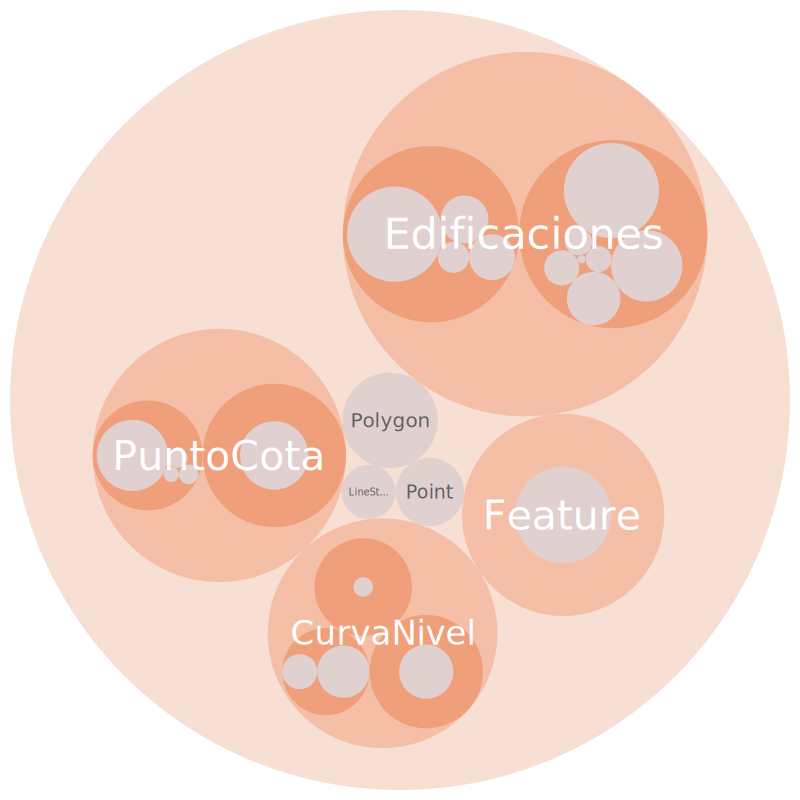
\includegraphics[width=0.7\linewidth]{imagenes/capitulo4/class-hierarchy-TFM}
	\caption{}
	\label{fig:class-hierarchy-tfm}
\end{figure}


\begin{figure}[H]
	\centering
	\includegraphics[width=0.7\linewidth]{imagenes/capitulo4/class-hierarchy-TFM-2}
	\caption{}
	\label{fig:class-hierarchy-tfm-2}
\end{figure}

\begin{figure}[H]
	\centering
	\includegraphics[width=0.7\linewidth]{imagenes/capitulo4/class-hierarchy-TFM-3}
	\caption{}
	\label{fig:class-hierarchy-tfm-3}
\end{figure}

\begin{figure}[H]
	\centering
	\includegraphics[width=0.7\linewidth]{imagenes/capitulo4/class-hierarchy-TFM-4}
	\caption{}
	\label{fig:class-hierarchy-tfm-4}
\end{figure}





Para entrar en contacto con las consultas de SPARQL y GeoSPARQL, vamos a recordar unas cuantas cosas.

Lo primero, disponemos de la información geográfica espacial referente a Ogíjares con respecto edificaciones, curvas de nivel y cotas de altura. Con esta información, que fue seleccionada para un fin, queremos saber las edificaciones que se encuentran a una cierta altura con el fin de obtener un objetivo, para ello, hemos cogido dos geometrías que nos pueden dar la misma aproximacion pero con geometrías distintas, una con puntos y otra con líneas.



\begin{lstlisting}
PREFIX rdf: <http://www.w3.org/1999/02/22-rdf-syntax-ns#>
PREFIX owl: <http://www.w3.org/2002/07/owl#>
PREFIX my: <http://example.org/ApplicationSchema#>
PREFIX geo: <http://www.opengis.net/ont/geosparql#>
PREFIX geosparql: <http://www.opengis.net/ont/geosparql#>

SELECT ?x ?p
WHERE {
?x rdf:type geo:EDI .
?polygon geo:asWKT ?p
}
LIMIT 3
\end{lstlisting}

\begin{figure}[H]
	\centering
	\includegraphics[width=0.7\linewidth]{imagenes/capitulo4/salida3}
	\caption{}
	\label{fig:salida3}
\end{figure}



\begin{lstlisting}
PREFIX rdf: <http://www.w3.org/1999/02/22-rdf-syntax-ns#>
PREFIX owl: <http://www.w3.org/2002/07/owl#>
PREFIX my: <http://example.org/ApplicationSchema#>
PREFIX geo: <http://www.opengis.net/ont/geosparql#>
PREFIX sf: <http://www.opengis.net/ont/sf#>
PREFIX xsd: <http://www.w3.org/2001/XMLSchema#>

SELECT ?f

WHERE {
?f geo:tieneCota ?fWKT
FILTER (?fWKT > 700)
}
LIMIT 5
\end{lstlisting}


\begin{figure}[H]
	\centering
	\includegraphics[width=0.7\linewidth]{imagenes/capitulo4/salida4}
	\caption{}
	\label{fig:salida4}
\end{figure}


\begin{lstlisting}
        PREFIX my: <http://example.org/ApplicationSchema#>
PREFIX geo: <http://www.opengis.net/ont/geosparql#>
SELECT DISTINCT ?point ?pointWKT ?pointCOTA
WHERE 
{
# Obtenemos todos los puntos con una cota determinada (> 720)
?point 	geo:asWKT ?pointWKT ;
geo:tieneCota ?pointCOTA .
FILTER (xsd:double(?pointCOTA) > 720)
}
LIMIT 3
\end{lstlisting}


\begin{figure}[H]
	\centering
	\includegraphics[width=0.7\linewidth]{imagenes/capitulo4/salida6}
	\caption{}
	\label{fig:salida6}
\end{figure}



Hay que tener en cuenta que hay muchas maneras de hacer las consultas, por lo que para obtener una cosa, no es necesario realizar la misma consulta,como acabamos de comprobar.

\begin{lstlisting}
PREFIX my: <http://example.org/ApplicationSchema#>
PREFIX geo: <http://www.opengis.net/ont/geosparql#>

PREFIX rdf: <http://www.w3.org/1999/02/22-rdf-syntax-ns#>

SELECT DISTINCT ?point ?pointCota
WHERE {
# Obtenemos todos los puntos con una cota determinada (> 720)
?point rdf:type geo:DEP ;
geo:tieneCota ?pointCota ;

FILTER (?pointCota > 700)
}
ORDER BY DESC(?pointCota)
LIMIT 5
\end{lstlisting}

\begin{figure}[H]
	\centering
	\includegraphics[width=0.7\linewidth]{imagenes/capitulo4/salida5}
	\caption{}
	\label{fig:salida5}
\end{figure}


\underline{GEOF:sfEquals}

\begin{lstlisting}
PREFIX my: <http://example.org/ApplicationSchema#>
PREFIX geo: <http://www.opengis.net/ont/geosparql#>
PREFIX geof: <http://www.opengis.net/def/function/geosparql/>

SELECT ?f
WHERE {
?f geo:asWKT ?fWKT .
FILTER (geof:sfEquals(?fWKT, '''
LINESTRING (440972.52 4106237.28,440972.4 4106232.04,440972.15 4106226.75,440967.68 4106204.44,440964.32 4106205.94,440963.48 4106208.23,440962.08 4106213.03,440960.59 4106219.28,440959.9 4106224.26,440958.99 4106229.78,440958.44 4106234.81,440958.11 4106240.01,440958.05 4106245.3,440958.04 4106250.86,440958.16 4106255.93,440958.41 4106261.44,440959.21 4106266.96,440960.76 4106272.24,440971.61 4106288.61,440974.39 4106281.06,440974.85 4106275.81,440974.77 4106270.3,440972.52 4106237.28)
'''^^geo:wktLiteral))
} 
\end{lstlisting}

\begin{figure}[H]
	\centering
	\includegraphics[width=0.7\linewidth]{imagenes/capitulo4/salida1}
	\caption{}
	\label{fig:salida1}
\end{figure}


\begin{lstlisting}
<!-- http://www.opengis.net/ont/geosparql#172684 -->

<owl:NamedIndividual rdf:about="http://www.opengis.net/ont/geosparql#172684">
<rdf:type rdf:resource="http://www.opengis.net/ont/geosparql#CGN"/>
<rdf:type rdf:resource="http://www.opengis.net/ont/geosparql#CMB"/>
<rdf:type rdf:resource="http://www.opengis.net/ont/geosparql#GID"/>
<rdf:type rdf:resource="http://www.opengis.net/ont/geosparql#NOR"/>
<rdf:type rdf:resource="http://www.opengis.net/ont/sf#LineString"/>
<geo:asWKT rdf:datatype="http://www.opengis.net/ont/geosparql#wktLiteral">LINESTRING (440972.52 4106237.28,440972.4 4106232.04,440972.15 4106226.75,440967.68 4106204.44,440964.32 4106205.94,440963.48 4106208.23,440962.08 4106213.03,440960.59 4106219.28,440959.9 4106224.26,440958.99 4106229.78,440958.44 4106234.81,440958.11 4106240.01,440958.05 4106245.3,440958.04 4106250.86,440958.16 4106255.93,440958.41 4106261.44,440959.21 4106266.96,440960.76 4106272.24,440971.61 4106288.61,440974.39 4106281.06,440974.85 4106275.81,440974.77 4106270.3,440972.52 4106237.28)</geo:asWKT>
<geo:tieneCota rdf:datatype="http://www.w3.org/2001/XMLSchema#double">780.0</geo:tieneCota>
</owl:NamedIndividual>
\end{lstlisting}


\begin{lstlisting}
PREFIX my: <http://example.org/ApplicationSchema#>
PREFIX geo: <http://www.opengis.net/ont/geosparql#>
PREFIX geof: <http://www.opengis.net/def/function/geosparql/>

SELECT ?f
WHERE {
?f geo:asWKT ?fWKT .
FILTER (geof:sfEquals(?fWKT, '''
POLYGON ((446050.16 4107127.71,446053.42 4107107.66,446029.09 4107103.93,446028.94 4107104.69,446027.13 4107112.67,446041.35 4107115.08,446039.91 4107125.24,446050.16 4107127.71))
'''^^geo:wktLiteral))
} 
\end{lstlisting}

\begin{figure}[H]
	\centering
	\includegraphics[width=0.7\linewidth]{imagenes/capitulo4/salida2}
	\caption{}
	\label{fig:salida2}
\end{figure}

\begin{figure}[H]
	\centering
	\includegraphics[width=0.7\linewidth]{imagenes/capitulo4/info-salida}
	\caption{}
	\label{fig:info-salida}
\end{figure}


\begin{lstlisting}
    <!-- http://www.opengis.net/ont/geosparql#181064 -->

<owl:NamedIndividual rdf:about="http://www.opengis.net/ont/geosparql#181064">
<rdf:type rdf:resource="http://www.opengis.net/ont/geosparql#EDI"/>
<rdf:type rdf:resource="http://www.opengis.net/ont/geosparql#GID"/>
<rdf:type rdf:resource="http://www.opengis.net/ont/geosparql#USO"/>
<rdf:type rdf:resource="http://www.opengis.net/ont/sf#Polygon"/>
<geo:asWKT rdf:datatype="http://www.opengis.net/ont/geosparql#wktLiteral">POLYGON ((446050.16 4107127.71,446053.42 4107107.66,446029.09 4107103.93,446028.94 4107104.69,446027.13 4107112.67,446041.35 4107115.08,446039.91 4107125.24,446050.16 4107127.71))</geo:asWKT>
</owl:NamedIndividual>
\end{lstlisting}

\underline{GEOF:WITHIN}

\begin{lstlisting}
PREFIX my: <http://example.org/ApplicationSchema#>
PREFIX geo: <http://www.opengis.net/ont/geosparql#>
PREFIX geof: <http://www.opengis.net/def/function/geosparql/>

PREFIX rdfs: <http://www.w3.org/2000/01/rdf-schema#>
SELECT ?f
WHERE {
?f geo:asWKT ?fWKT .
FILTER (geof:sfEquals(?fWKT, '''
MULTIPOINT ((446228.92 4108432.53))
'''^^geo:wktLiteral))
} 


\end{lstlisting}

\begin{figure}[H]
	\centering
	\includegraphics[width=0.7\linewidth]{imagenes/capitulo4/salida7}
	\caption{}
	\label{fig:salida7}
\end{figure}


geof:distance

Find the 3 closest features to feature my:C, where computations are based on my:hasExactGeometry.

\begin{lstlisting}
PREFIX uom: <http://www.opengis.net/def/uom/OGC/1.0/>
PREFIX my: <http://example.org/ApplicationSchema#>
PREFIX geo: <http://www.opengis.net/ont/geosparql#>
PREFIX geof: <http://www.opengis.net/def/function/geosparql/>

SELECT ?f
WHERE {
geo:889549 geo:asWKT ?WKT .
?f geo:asWKT ?fWKT .
FILTER (?fGeom != ?WKT)
}

ORDER BY ASC(geof:distance(?cWKT, ?fWKT, uom:metre))
LIMIT 5
\end{lstlisting}

\begin{figure}[H]
	\centering
	\includegraphics[width=0.7\linewidth]{imagenes/capitulo4/salida8}
	\caption{}
	\label{fig:salida8}
\end{figure}


\begin{lstlisting}
PREFIX uom: <http://www.opengis.net/def/uom/OGC/1.0/>
PREFIX my: <http://example.org/ApplicationSchema#>
PREFIX geo: <http://www.opengis.net/ont/geosparql#>
PREFIX geof: <http://www.opengis.net/def/function/geosparql/>
PREFIX rdf: <http://www.w3.org/1999/02/22-rdf-syntax-ns#>
PREFIX sf: <http://www.opengis.net/ont/sf#>

SELECT ?f
WHERE {
geo:889549 geo:asWKT ?WKT .

?f rdf:type sf:Point ;
geo:asWKT ?fWKT .
FILTER (?fGeom != ?WKT)
}

ORDER BY ASC(geof:distance(?cWKT, ?fWKT, uom:metre))
LIMIT 5
\end{lstlisting}

\begin{figure}[H]
	\centering
	\includegraphics[width=0.7\linewidth]{imagenes/capitulo4/salida9}
	\caption{}
	\label{fig:salida9}
\end{figure}

\begin{lstlisting}
PREFIX uom: <http://www.opengis.net/def/uom/OGC/1.0/>
PREFIX my: <http://example.org/ApplicationSchema#>
PREFIX geo: <http://www.opengis.net/ont/geosparql#>
PREFIX geof: <http://www.opengis.net/def/function/geosparql/>
PREFIX rdf: <http://www.w3.org/1999/02/22-rdf-syntax-ns#>
PREFIX sf: <http://www.opengis.net/ont/sf#>

SELECT ?f
WHERE {
geo:889549 geo:asWKT ?WKT .

?f rdf:type sf:LineString ;
geo:asWKT ?fWKT .
FILTER (?fGeom != ?WKT)
}

ORDER BY ASC(geof:distance(?cWKT, ?fWKT, uom:metre))
LIMIT 5
\end{lstlisting}

\begin{figure}[H]
	\centering
	\includegraphics[width=0.7\linewidth]{imagenes/capitulo4/salida10}
	\caption{}
	\label{fig:salida10}
\end{figure}

\begin{lstlisting}
PREFIX uom: <http://www.opengis.net/def/uom/OGC/1.0/>
PREFIX my: <http://example.org/ApplicationSchema#>
PREFIX geo: <http://www.opengis.net/ont/geosparql#>
PREFIX geof: <http://www.opengis.net/def/function/geosparql/>
PREFIX rdf: <http://www.w3.org/1999/02/22-rdf-syntax-ns#>
PREFIX sf: <http://www.opengis.net/ont/sf#>

SELECT ?p
WHERE {
?p rdf:type sf:Polygon ;
geo:asWKT ?pWKT .

?f rdf:type sf:Point ;
geo:tieneCota ?pointCota ;
geo:asWKT ?fWKT .

FILTER (?pointCota > 700)

}

ORDER BY ASC(geof:distance(?pWKT, ?fWKT, uom:metre))
LIMIT 5
\end{lstlisting}

\begin{figure}[H]
	\centering
	\includegraphics[width=0.7\linewidth]{imagenes/capitulo4/salida11}
	\caption{}
	\label{fig:salida11}
\end{figure}



geo:sfContains



\subsection{Visualización de la Información Geográfica}


Sin embargo, con eso sólo podemos obtener los identificadores que queremos, ¿entonces como podemos visualizarlo y ubicarlos en un mapa?

La respuesta es muy simple con Leaflet.



\section{Evaluación de la prueba de concepto}





\newpage





%Gracias a este tipo de archivo podemos generar MDT secundarios: mapas de orientación, de pendiente, cuencas visuales o sencillos archivos de sombreado (\textit{hillshade}), materia prima con la que analizar el territorio. Es por ello que, una vez descargados nuestros datos, ya podemos llevar a cabo el análisis del mapa de sombras para el MDT. Primero lo realizaremos en R, seguidamente en QGIS y, por último, veremos la interacción entre ambas, dejando documentado el proceso, para así poder hacer la evaluación y comparación entre ambas herramientas.





\newpage

% Uso de la similitud semántica para la recuperación de información geoespacial: https://dialnet.unirioja.es/servlet/tesis?codigo=61960
% http://rua.ua.es/dspace/handle/10045/45811
% https://rua.ua.es/dspace/bitstream/10045/45811/1/tesis_machado_garcia.pdf

% http://www.ciw.cl/material/tw07arodriguez.pdf

% Semántica Geoespacial en la web: https://slideplayer.es/slide/10277009/

% https://nextweb.gnoss.com/busqueda/tag/geoespacial

% Para que es para acceder a datos espaciales en la web
% http://linkedgeodata.org/OnlineAccess
% http://linkedgeodata.org/sparql

% https://www.w3.org/community/geosemweb/wiki/Main_Page
% https://en.wikipedia.org/wiki/Semantic_Geospatial_Web
% https://www.opengeospatial.org/projects/initiatives/gswie
% http://www.personal.psu.edu/faculty/f/u/fuf1/Fonseca-Sheth.pdf

% https://www.researchgate.net/publication/283801501_Geospatial_Semantic_Web
% https://www.researchgate.net/publication/300494545_Geospatial_Data_Interoperability_Geography_Markup_Language_GML_Scalable_Vector_Graphics_SVG_and_Geospatial_Web_Services
% https://www.semanticscholar.org/paper/Supporting-Frameworks-for-the-Geospatial-Semantic-Abdelmoty-Smart/e3998c31905b0d9eebaceddad5040e940caa594a
% https://www.sciencedirect.com/science/article/pii/S1570826809000468

% https://www.mdpi.com/journal/ijgi/special_issues/geospatial_semantics

% Documentos Scholar sobre "geospatial semantic web": https://scholar.google.es/scholar?q=geospatial+semantic+web&hl=es&as_sdt=0&as_vis=1&oi=scholart

% http://www.irisa.fr/LIS/ferre/sparklis/?title=Core%20English%20DBpedia&endpoint=http%3A//servolis.irisa.fr/dbpedia/sparql&sparklis-query=%5BVId%5DReturn%28Det%28An%281%2CModif%28Select%2CUnordered%29%2CClass%28%22http%3A//dbpedia.org/ontology/Database%22%29%29%2CNone%29%29&sparklis-path=D
% http://www.irisa.fr/LIS/ferre/sparklis/?endpoint=http%3A//servolis.irisa.fr/dbpedia/sparql&sparklis-query=%5BVId%5DReturn%28Det%28An%287%2CModif%28Select%2CUnordered%29%2CClass%28%22http%3A//dbpedia.org/ontology/Place%22%29%29%2CNone%29%29&sparklis-path=D

% https://www.sciencedirect.com/science/article/pii/S1570826809000468

% http://www.geonames.org/ontology/documentation.html

% https://ieeexplore.ieee.org/document/1656068

% https://www.chnt.at/the-geospatial-semantic-web-as-foundation-for-knowledge-networks-of-cultural-heritage/

% http://geoknow.eu/Welcome.html


%Un SIG ha sido ampliamente utilizado por una variedad de aplicaciones, muchas bases de datos geográficas han sido desarrolladas por diferentes programas y software. Sin embargo, sigue siendo un gran problema compartir estos datos geoespaciales y usarlos para el desarrollo de aplicaciones SIG. No es que los datos no estén disponibles, hay una gran cantidad de datos geográficos almacenados en diferentes lugares y en diferentes formatos, pero la reutilización de datos para nuevas aplicaciones y el intercambio de datos son tareas abrumadoras debido a la heterogeneidad de los sistemas existentes en términos de conceptos de modelado de datos, técnicas de codificación de datos y estructuras de almacenamiento, etc.\\

%Hay dos problemas que resultan directamente de la no interoperabilidad de las bases de datos. Uno es el cambio en la exactitud de los datos. Después de que los datos se conviertan de un formato a otro, pueden ocurrir problemas como la precisión de coordenadas, errores de omisión, nombres de atributos faltantes o incorrectos y una topología incorrecta. El segundo problema es la inversión de tiempo y dinero para la conversión de datos. Se ha desperdiciado mucho dinero y tiempo en la conversión de datos o en el desarrollo de herramientas de conversión de datos.\\

%La interoperabilidad de datos significa la capacidad de utilizar una variedad de formatos de datos. Los datos geoespaciales interoperables pueden ser utilizados por diferentes tipos de programas y aplicaciones. Con datos geoespaciales interoperables, los usuarios deben poder solicitar, acceder e integrar datos fácilmente sin importar dónde se almacenen los datos (local o remotamente). La interoperabilidad de los datos geoespaciales es extremadamente importante para las aplicaciones geoespaciales, ya que existían grandes cantidades de datos espaciales de diferentes formatos geográficos y hay una mayor demanda de reutilización de estos datos espaciales existentes para la toma de decisiones. La interoperabilidad de los datos geoespaciales elimina las barreras para el intercambio de datos y permite a los usuarios acceder, mapear, visualizar y analizar directamente datos con diferentes formatos de datos espaciales. Los datos geoespaciales interoperables hacen posible la distribución rápida de información y el intercambio entre departamentos.\\


%\section{Web Semántica Geoespacial}

% http://www.mclibre.org/consultar/xml/lecciones/web-semantica.html#spatial-data

%\subsection{Arquitectura Web Semántica Geoespacial}

% se debería de hacer una mención a la web semántica tradicional o la web tradicional


% 

https://mangomap.com/gis-mapping

% ---------------------------------------------------------------------------

%¿qué datos cogemos?
%
%Descargamos datos de aquí: https://www.juntadeandalucia.es/institutodeestadisticaycartografia/bcadescargas/
%- Base Cartográfica de Andalucía (2) > Base Cartográfica de Andalucía (shape) > Ogíjares
%
%Para saber más información acerca de los datos: https://www.juntadeandalucia.es/institutodeestadisticaycartografia/prodCartografia/bc/modelo.htm
%
%Para instalar Google Maps en QGIS
%https://mappinggis.com/2018/03/como-anadir-mapas-base-en-qgis-3-0-openstreetmap-google-carto-stamen/
%
%
%- Elemento Edificaciones (poligonal): Se agrupan en esta capa varios elementos que conforman edificaciones. Se debe tener en cuenta que el nucleo urbano engloba en áreas grandes a las edificaciones.
%
%- Elemnto ParqueJardinP (puntual): Recinto en el interior de una población destinado a prados, jardines y arbolado
%para recreo y ornato. 

%-----

%Se trabajará con información  geoespacial, concretamente con archivos en formato Shapefile. 
%
%La mejora de las herramientas se enfocará únicamente a las destinadas a la generación (QGIS que permitirá llevar la información  de los shapefile hacia hojas de cálculo y Protegé permitirá llevar la información  de los shapefile hacia documentos en formato RDF), y consumo GraphBD que permite la visualización de archivos en formato RDF y visualización (aplicación en R que permite la visualización de archivos en formato RDF),  y como lenguaje de consulta geoespacial, este estándar es GEOSPARQL.
%
%Finalmente, todos los datos generados mediante las herramientas mejoradas, se publicarán en un repositorio disponible, el cual dará lugar al: repositorio de Datos Enlazados Ecuatoriano el cual debe permitir su acceso al público en general. 


% ----

%Para hacer uso de este lenguaje de consulta, es necesario utilizar herramientas que permitan GeoSPARQL, no sólo SPARQL. Es por eso que la herramienta Protegé carece de funcionamiento para este tipo de consultas
%
%Como hemos comentado anteriormente, la herramienta Protegé nos permite construir contologías de manera más sencilla y rápida, sin embargo, también nos ofrece herramienta para realizar consultas con SPARQL. No obstante, carece de funcionamiento para las consultas de GeoSPARQL. En el siguiente apartado, hablaremos también 
%
%en este caso, 

%---

\section{Resumen del capítulo}






%% Realizar el mismo ejemplo en ambos y comparar mejoras, deficiencias de cada uno, diferencias..

\chapter{Resultados}
\label{ch:resultados}

\begin{quote}
  {\bf\textsc{Resumen:}} Este capítulo ...
\end{quote}


\section{Resumen del capítulo}








%% La conclusión debe contener los principales aspectos y contribuciones para finalizar el trabajo presentado. Se debe presentar lo que se esperaba del trabajo a través de los objetivos introducidos inicialmente y mostrar lo que se logró. No se debe insertar un nuevo asunto en la conclusión. Aquí el autor presentará las propias impresiones sobre el trabajo efectuado. Es importante también que se identifiquen limitaciones y problemas que surgieron durante el desarrollo del trabajo y cuáles las consecuencias del mismo.

% Los trabajos futuros deben contener oportunidades de expansión del trabajo presentado, así como nuevos proyectos que pudieron ser vislumbrados a partir del desarrollo del trabajo.

\chapter{Conclusiones y Trabajo Futuro}
\label{ch:Conclusiones y Trabajo Futuro}

\begin{quote}
  {\bf\textsc{Resumen:}} Este capítulo recoge los principales aspectos y contribuciones obtenidos para la integración de Información Geográfica en la Web Semántica. De igual manera, comprobaremos el cumplimiento de los objetivos que introducimos inicialmente en el \texttt{capítulo 1}. Asimismo, se comentarán posibles propuestas de mejora de cara a posibles iteraciones del proyecto, además de comentar otras posibles aplicaciones relacionadas, que caen fuera del ámbito de este trabajo.
\end{quote}




\section{Conclusiones}

En este TFM se ha profundizado en el uso de la Web Semántica Geoespacial, en concreto en la posibilidad de integrar Información Geográfica en la Web Semántica mediante el uso de herramientas específicas, a través de la creación de la ontología GEOARES. Se han estudiado algunas de las tecnologías que se pueden utilizar para representar e integrar Información Geográfica, como los lenguajes de ontologías (RDF, OWL) y de consultas (SPARQL y GeoSPARQL). Se han valorado las herramientas de la Web Semántica para permitir crear la ontología, como GraphDB y Protegé, esta última no ha permitido incluir el \textit{plugin} de GeoSPARQL, no obstante, la alternativa encontrada, GraphDB, ha permitido solventar los problemas ocasionados con Protegé. \\

Así, se ha desarrollado una prueba de concepto trabajando con información geoespacial, concretamente con archivos en formato \textit{Shapefile} de la provincia de Granada, en particular de mi pueblo, Ogíjares, y centrándonos en la información geoespacial obtenida de edificaciones, puntos de cota y curvas de nivel, para su integración en la ontología y su posterior visualización en un mapa a través de R. Dentro de todas las posibilidades de análisis que ofrece la Web Semántica, se ha prestado especial atención a la relacionada con Información Geográfica, en donde, gracias a los estándares definidos, es decir, las funciones usadas en GeoSPARQL, las cuales son las mismas que OGC ha definido en su estándar para el tratamiento de datos SIG, es posible combinar dos ámbitos que previamente parecían ser independientes el uno respecto del otro. Entonces, se han utilizado tecnologías tanto de la Web Semática como de los SIG que nos allanan el camino para ambas áreas, permitiendo la heterogeneidad e interoperabilidad de los datos geográficos gracias a la capa semántica que estos presentan.\\


%Se ha apreciado, que las funciones usadas en el GeoSPARQL son las mismas que OGC ha definido en su estándar. Con esto acabamos de comprobar como ha sido posible unir dos ámbitos que previamente parecían ser independientes el uno respecto del otro.
A la vista de los resultados obtenidos, considero que haber realizado esta prueba de concepto me ha abierto nuevos puntos de vista hacia otra perspectiva de la Web. Parte de mi contribucción ha sido enseñar las herramientas que facilitan el trabajo para la puesta en marcha de una ontología. Por tanto, mediante el desarrollo de este TFM, valoro que se han conseguido los objetivos señalados en la \texttt{subsección \ref{ch:objetivos}} del \texttt{capítulo \ref{ch:introduccion}}, en concreto:


\begin{enumerate}
	
	\item Se ha mostrado mediante la utilización de la Web Semántica Geoespacial, cómo los estándares que se usan en el lenguaje de consulta geoespacial corresponden a los mismos definidos por el organismo OGC para los datos geográficos (ver \texttt{capítulo \ref{ch:capitulo4}}).
	%\item \textbf{Comprender la relación existente entre los Sistemas de Información Geográfica y la Web Semántica}, a priori dos áreas completamente diferentes.
	
	\item Se han definido dos fuentes principales de información con las que obtener datos públicos geográficos de buena calidad y se han usado los datos de una de ellas, en concreto los del Instituto de Estadística y Cartografía de Andalucía (ver \texttt{sección \ref{ch:capitulo5-datos}}).
	
	%\item \textbf{Hacer uso de fuentes de información geoespacial}, con las que obtener datos públicos geográficos de buena calidad.
	
	\item Se han considerado herramientas de la Web Semántica de gran alcance para representar e integrar Información Geográfica, entre las que destacamos Protegé y GraphDB (ver \texttt{capítulo \ref{ch:capitulo5}}).
	%\item \textbf{Localizar diversas herramientas de la Web Semántica} que se puedan utilizar para representar e integrar Información Geográfica.
	
	\item Se ha mostrado mediante Protegé cómo es posible agregar conocimiento de dominio geoespacial sobre la estructura de los datos de manera sencilla (ver \texttt{sección \ref{ch:crear}}).
	%\item Aprender a \textbf{agregar conocimiento de dominio geoespacial sobre la estructura de los datos} mediante el empleo de herramientas de la Web Semántica como Protegé.
	
	\item Se ha mostrado mediante Protegé cómo es posible poblar una ontología de manera eficaz haciendo uso de diversas reglas (ver \texttt{sección \ref{ch:poblar}}).
	%\item \textbf{Aprender a crear ontologías y poblarlas}  mediante información geográfica existente.
	
	\item Se ha realizado un estudio acerca de las carencias o mejoras que supone usar Protegé (ver \texttt{Apéndice \ref{ch:ApendiceB}}).
	%\item Apreciar las carencias o mejoras que supone usar \textbf{Protegé frente a otro tipo de herramientas}.
	
	\item Se han mostrado la estructura de los datos geoespaciales y sus especificaciones para realizar consultas con el lenguaje GeoSPARQL (ver \texttt{sección \ref{ch:capitulo4-geosparql}} y \texttt{sección \ref{ch:consultas}}).
	%\item Conocer cuál es la \textbf{estructura de los datos geoespaciales y sus especificaciones para realizar consultas con el lenguaje GeoSPARQL}.
	
	\item Se ha aprendido a crear un mapa Web en R mediante el uso de la biblioteca \textit{Leaflet} y el framework \textit{Shiny} para ubicar información geoespacial en un mapa (ver \texttt{sección \ref{ch:visualizacion}}).
	%\item Aprender a \textbf{ubicar información geoespacial en un mapa mediante el uso de la biblioteca Leaflet}.
	
	\item Se ha mostrado, mediante ejemplos, formas de trabajo sobre la Web Semántica Geoespacial (ver \texttt{capítulo \ref{ch:capitulo5}}).
	%\item Mostrar algunos \textbf{métodos de trabajo}, estrechamente adaptados al tratamiento de Información Geográfica en la Web Semántica.
	
	\item Se ha prestado especial atención a desarrollar un trabajo autocontenido, tratando que sea accesible a cualquier persona con un perfil tecnológico básico que esté interesado en el tema.
	
	%\item \textbf{Aportaciones a la comunidad o al lector}, para que el proyecto sirva como puerta de acceso al mundo de la Web Semántica y en particular, al de la Web Semántica Geoespacial, y facilite el acceso a parte de los conocimientos actuales disponibles.
	
	\item He adquirido experiencia y conocimientos en un tema nuevo para mí, la Web Semántica, y ampliado otros como el caso de los Sistemas de Información Geográfica.
	%\item \textbf{Aportaciones hacia mi persona} en la puesta en práctica y adquisición de conocimiento de los anteriores puntos.
	%\item \textbf{Aportaciones hacia mi persona} en la adquisición de conocimientos de la Web Semántica, creación de ontologías, manejo de herramientas semánticas como Protegé y aprendizaje para la creación de un mapa interactivo mediante la librería Shiny de R.	
	
	

	
\end{enumerate}



%La WS es aún una visión, un proyecto de futuro muy ambicioso, que permitirá, con ayuda de la Inteligencia Artificial, realizar un sinfín de operaciones en la Web, mucho más amplias que las ofertadas hoy en día. El tener toda la información etiquetada sintáctica y semánticamente facilitará la implementación eficaz de los llamados agentes inteligentes, capaces de ofrecer información Web pertinente, en función de los intereses y circunstancias personales de cada usuario (personalización máxima).



%Esta situación imaginaria tiene ya su base real, materializada en los proyectos piloto realizados y en los grandes avances logrados para su creación en cuanto a estándares e infraestructura. Las principales empresas, como IBM, Microsoft, etc. participan activamente en su desarrollo, así como la comunidad investigadora, especialmente la universitaria. Por supuesto, el proyecto no hubiera sido posible sin el apoyo e impulso de la W3C, que junto con el sitio oficial www.semanticweb.org, se encarga de ofrecer toda la información disponible sobre los progresos en este ámbito. El interés por la WS se refleja en la celebración anual del Congreso internacional de la WWW, que en 2009 ha tenido lugar en la Universidad Politécnica de Madrid. También queda patente con la publicación de la revista Journal of Web Semantics.

%En el terreno de las bibliotecas, la WS podrá ser decisiva de cara a la construcción de una Biblioteca Digital Universal, donde todo sea accesible de forma rápida y precisa, se encuentre donde se encuentre. Por supuesto, aún queda mucho camino por recorrer y la transición de la Web actual a la WS puede implicar un coste altísimo (en tiempo, dinero y esfuerzo), ya que no sólo se trata de estructurar la información web venidera, sino también la ya existente, labor que se prevé irrealizable.

\section{Proyectos relacionados}

Dentro de los proyectos relacionados con la Web Semántica y los SIG, destacan los documentados en el libro \textit{\textbf{Geospatial Semantic Web}} de \textit{Chuanrong Zhang}, \textit{Tian Zhao} y \textit{Weidong Li}. Este libro cubre temas clave relacionados con la Web Semántica Geoespacial; ontología geoespacial para la interoperabilidad semántica; creación, intercambio e integración de ontologías; desafíos de la Web Semántica Geoespacial; desarrollo de aplicaciones Web Semánticas Geoespaciales, entre otros. Asimismo, se describen tecnologías, como WFS, WMS, RDF, OWL y GeoSPARQL, y muestra cómo usar las tecnologías de la Web Semántica Geoespacial para resolver problemas prácticos del mundo real, como los datos espaciales \cite{libro-gis}. \\

También son remarcables los trabajos siguientes: ``La Web semántica y las tecnologías del lenguaje humano'' en \cite{researchgate}, ``Geography 2.0—A mash-up perspective'' \cite{gml} y ``Data Models and Query Languages for Linked Geospatial Data'' en \cite{wkt-database}; en donde se cubren las áreas de la Web Semántica, SIG y la combinación de ambas, entre otros.\\

Por otro lado, destacar un proyecto de la Universidad de Almería \textbf{XOSM}, \textit{XQuery for OpenStreetMap} (\url{http://xosm.ual.es/XOSM/query.php}), que hace uso de la Información Geográfica Voluntaria mediante OpenStreetMap (OSM) para ofrecer datos de mapas urbanos y rurales. XOSM es una herramienta para el procesamiento de consultas geoespaciales en OSM equipada con un lenguaje de consulta basado en un conjunto de operadores definidos para OSM implementados como una biblioteca del lenguaje de consulta \textit{XML XQuery}. Esta biblioteca proporciona un repertorio de funciones espaciales que actúan sobre la representación XML de una capa OSM y permite la definición de consultas que combinan capas OSM y capas creadas a partir de recursos de datos abiertos vinculados (KML, GeoJSON, CSV y RDF). \\

En la figura \ref{fig:1-6} se puede observar la página de inicio de esta herramienta, en donde, explica en que consiste. 


% COMENTAR FIGURAS


%LOs datos se crean con KML (xosm.ual.es)

\begin{figure}[H]
	\centering
	\includegraphics[width=1\linewidth]{imagenes/capitulo6/1}
	\caption{Página de inicio de XOSM}
	\label{fig:1-6}
\end{figure}

Por otro lado, las figuras \ref{fig:2-6} y \ref{fig:3-6} nos muestran un ejemplo del funcionamiento de XOSM en donde se representan en un mapa las calles de Londres que cruzan la calle \textit{Haymarket} y tocan \textit{Trafalgar Square}.

\begin{figure}[H]
	\centering
	\includegraphics[width=1\linewidth]{imagenes/capitulo6/2}
	\caption{Hacer consulta en XOSM}
	\label{fig:2-6}
\end{figure}

\begin{figure}[H]
	\centering
	\includegraphics[width=1\linewidth]{imagenes/capitulo6/3}
	\caption{Salida de una consulta de ejemplo en XOSM}
	\label{fig:3-6}
\end{figure}


Y cómo se observa, este TFM se mantiene en la línea de estos proyectos.

\section{Trabajo futuro}

Durante la realización de este TFM se han encontrado o han podido surgir temas, ejemplos o aplicaciones bastantes relacionados pero que no se han estudiado en el mismo, por este motivo, comentaremos algunos aspectos a profundizar en el futuro:

\begin{enumerate}
	
	\item Crear una plataforma parecida a la mostrada en las figuras \ref{2-6} y \ref{fig:3-6}, en donde, a partir de la salida de la consulta que se haga, obtener el GID ubicado automáticamente en el mapa, es decir, integrar en una herramienta la prueba de concepto realizada.
	
	\item Generar otro ejemplo con la misma Información Geográfica pero obtenida de otra parte, para comprobar cómo la Web Semántica, gracias a su estructura, permite la heterogeneidad.
	
	%\item Generar modelos para obtener la temperatura de una superficie a partir de la altitud y la localización del territorio.
	%\item Realizar un estudio con la función $terrain$ de R para la rugosidad del terreno, ya que dicha función no sólo permite obtener la pendiente y la orientación, sino otras variables cartográficas.
	%\item Ampliar el paquete desarrollado para facilitar este tipo de análisis, así como, aumentar el volumen de datos cargados en la misma, centrándonos en los MDT de España.
\end{enumerate}

Adicionalmente, considero que este tema y el enfoque que le he dado puede tener interés para el público en general por lo que valoro la posibilidad de darle más difusión al trabajo.




%%%%%%%%%%%%%%%%%%%%%%%%%%%%%% ANEXO %%%%%%%%%%%%%%%%%%%%%%%%%%%%%

%\section*{\centering{A – ANEXOS Y APÉNDICES }} % Añadir código
%\addcontentsline{toc}{section}{A - ANEXOS Y APÉNDICES}

% Los anexos y apéndices son materiales adicionales, utilizados para complementar el texto, añadidos al final del trabajo, con la finalidad de aclaración o de comprobación. Son elaborados por el autor y pretenden complementar una argumentación y sirven de fundamentación teórica, comprobación e ilustración (por ejemplo, mapas, leyes, códigos)

%\chapter*{Apendice A - }
%\label{ch:Apendice}

%\section*{\huge Apéndice A} 
%\section*{Fuentes de información para la descarga de MDT}
%\addcontentsline{toc}{chapter}{Apéndice A: Fuentes de información para descarga de MDT}

%\begin{itemize}
%	\item \item \url{https://www.cursosteledeteccion.com/fuentes-gratuitas-para-descargar-dem-modelo-de-elevacion-digital/}
%	\item \url{http://www.gisandbeers.com/descarga-de-dem-mundiales-mde/}
%	\item \url{https://gisgeography.com/free-global-dem-data-sources/}
%	\item \url{http://www.gpsvisualizer.com/elevation}
%	\item \url{https://mappinggis.com/2017/12/programas-gratuitos-para-trabajar-con-imagenes-de-satelite/}
%\end{itemize}

\newpage

\chapter{Planificación del TFM}

%\section*{\huge Apéndice A} 
%\section*{Planificación del TFM}
\label{ch:ApendiceA}
%\addcontentsline{toc}{chapter}{Apéndice A: Planificación del TFM}

\begin{table}[H]
		\centering
		\rotatebox{90}{%   
	\begin{tabular}{|
			>{\columncolor[HTML]{EFEFEF}}c |l|l|l|l|l|}
		\hline
		\cellcolor[HTML]{C0C0C0}                                                           & \multicolumn{5}{c|}{\cellcolor[HTML]{C0C0C0}\textbf{TIEMPO}}                                                                                                                                                                                                                                                                                                                                                                                                                                                                                                                                                                                                                                                                                                                                               \\ \cline{2-6} 
		\multirow{-2}{*}{\cellcolor[HTML]{C0C0C0}\textbf{TAREAS}}                          & \multicolumn{1}{c|}{\cellcolor[HTML]{EFEFEF}{\color[HTML]{333333} \textit{Noviembre}}}                                                                    &  \multicolumn{1}{c|}{\cellcolor[HTML]{EFEFEF}{\color[HTML]{333333} \textit{Enero-Abril}}}                                                                   & \multicolumn{1}{c|}{\cellcolor[HTML]{EFEFEF}{\color[HTML]{333333} \textit{Junio-Julio}}}                            & \multicolumn{1}{c|}{\cellcolor[HTML]{EFEFEF}{\color[HTML]{333333} \textit{Agosto}}}                                                                    & \multicolumn{1}{c|}{\cellcolor[HTML]{EFEFEF}{\color[HTML]{333333} \textit{Septiembre}}}                        \\ \hline
		\begin{tabular}[c]{@{}c@{}}Elección \\ del tema\end{tabular}                       & \multicolumn{1}{c|}{\begin{tabular}[c]{@{}c@{}}Reuniones\\ con el tutor \end{tabular}} &                                                                                          &                                                                                                                                                           &                                                                                                               &                                                                                                                                                                                                                                                                        \\ \hline
		\begin{tabular}[c]{@{}c@{}}Búsqueda \\ de mapas\end{tabular}           &                                                                                                                                                           & \multicolumn{2}{c|}{\begin{tabular}[c]{@{}c@{}}Obtención de  \\ datos geoespaciales \end{tabular}}                                                               &                                                                                                               &                                                                                                                                                                                                                                                                        \\ \hline
		Documentar                                                            &                                                                                                                                                           &                                                                                          & \multicolumn{1}{c|}{\begin{tabular}[c]{@{}c@{}}Lectura \\ papers \end{tabular}} &                                                                                                                        \multicolumn{1}{c|}{\begin{tabular}[c]{@{}c@{}}Redacción de \\ los capítulos \end{tabular}}                                                                                                                         &                                                                                                                \\ \hline
		\begin{tabular}[c]{@{}c@{}}SIG\end{tabular}     &                                                                                                                                                           &                                                                                          & \multicolumn{1}{c|}{\begin{tabular}[c]{@{}c@{}}Repaso de \\ conceptos \end{tabular}}                                                                         &                                                                                                               &                                                                                                                                                                                                                                                                        \\ \hline
		\begin{tabular}[c]{@{}c@{}}Web\\ Semántica\end{tabular}                            &                                                                                                                                                           &                                                                                          &                                                                                                                                                           & \multicolumn{1}{c|}{\begin{tabular}[c]{@{}c@{}}Estudio de los\\ conceptos de la\\ Web Semántica\end{tabular}} &                                                                                                                                                                                                                                                                        \\ \hline
		\begin{tabular}[c]{@{}c@{}}Prueba de \\ concepto\end{tabular}                                                                                                                                                            &                                                                                          &                                                                                                                                                           & \multicolumn{2}{c|}{\begin{tabular}[c]{@{}c@{}}Creación de la ontología, \\ consultas y visualización\end{tabular}}                                                                                 & \multicolumn{1}{c|}{}                                                                                          \\ \hline
		Anexos                                                                             &                                                                                                                                                           &                                                                                          &                                                                                                                                                           &                                                                                                               & \multicolumn{1}{c|}{\begin{tabular}[c]{@{}c@{}}Agregación de \\ documentación a \\ temas poco tratados \end{tabular}}                                                                                                                 \\ \hline
		Conclusiones                                                                       &                                                                                                                                                           &                                                                                          &                                                                                                                                                           &                                                                                                                                                                                                                                                                       & \multicolumn{1}{c|}{\begin{tabular}[c]{@{}c@{}}Realización de \\ las conclusiones\end{tabular}}                \\ \hline
		\begin{tabular}[c]{@{}c@{}}Repaso y \\ entrega\end{tabular}                        &                                                                                                                                                           &                                                                                          &                                                                                                                                                                                                                                                                         &                                                                                                                                                        & \multicolumn{1}{c|}{\begin{tabular}[c]{@{}c@{}}Repaso para \\  su entrega\end{tabular}} \\ \hline
	\begin{tabular}[c]{@{}c@{}}Reuniones\end{tabular}                   & \multicolumn{5}{c|}{\begin{tabular}[c]{@{}c@{}}Durante todo el proceso he estado en contacto con el tutor del TFM\\  o bien a través de tutorías o bien a través del correo electrónico\end{tabular}}                                                                                                                                                                                                                                                                                                                                                                                                                                                                                                                                                  \\ \hline
	\end{tabular}}
\end{table}


% \usepackage{multirow}
% \usepackage{colortbl}
% \usepackage{hhline}


%En el anterior cronograma se contempla la planificación realizada para el desarollo del Trabajo de Fin de Máster. He de remarcar que durante el proceso he estado en contacto con el tutor del TFM o bien a través de tutorías o a través del correo electrónico.

%%%%%%%%%%%%%%%%%%%%%%%%%%%%%% ANEXO %%%%%%%%%%%%%%%%%%%%%%%%%%%%%

%\section*{\centering{A – ANEXOS Y APÉNDICES }} % Añadir código
%\addcontentsline{toc}{section}{A - ANEXOS Y APÉNDICES}

% Los anexos y apéndices son materiales adicionales, utilizados para complementar el texto, añadidos al final del trabajo, con la finalidad de aclaración o de comprobación. Son elaborados por el autor y pretenden complementar una argumentación y sirven de fundamentación teórica, comprobación e ilustración (por ejemplo, mapas, leyes, códigos)

%\chapter*{Apendice A - }
%\label{ch:Apendice}

%\section*{\huge Apéndice A} 
%\section*{Fuentes de información para la descarga de MDT}
%\addcontentsline{toc}{chapter}{Apéndice A: Fuentes de información para descarga de MDT}

%\begin{itemize}
%	\item \item \url{https://www.cursosteledeteccion.com/fuentes-gratuitas-para-descargar-dem-modelo-de-elevacion-digital/}
%	\item \url{http://www.gisandbeers.com/descarga-de-dem-mundiales-mde/}
%	\item \url{https://gisgeography.com/free-global-dem-data-sources/}
%	\item \url{http://www.gpsvisualizer.com/elevation}
%	\item \url{https://mappinggis.com/2017/12/programas-gratuitos-para-trabajar-con-imagenes-de-satelite/}
%\end{itemize}

\newpage


\chapter{Instalación de GraphDB}
%\section*{\huge Apéndice C} 
%\section*{Instalación de GraphDB}
\label{ch:ApendiceC}
%\addcontentsline{toc}{chapter}{Apéndice C: Instalación de GraphD}

%\chapter*{Apéndice B: Instalación de GraphD}
%\subsection{Tipos de Web} % Evolución de la Web

	
\textit{\textbf{Nota}: La instalación y uso de GraphDB se ha hecho en macOS 10.14}\\

\begin{figure}[H]
	\centering
	\begin{subfigure}[h]{0.78\textwidth} 
		\includegraphics[width=\textwidth]{imagenes/apendices/1}
		\caption{}
	\end{subfigure}       
	\begin{subfigure}[h]{0.78\textwidth} 
		\includegraphics[width=\textwidth]{imagenes/apendices/2}
		\caption{}
	\end{subfigure}
	\caption{Página para la descarga de GraphDB Free}
	\label{fig:1}
\end{figure}

\textbf{GraphDB} es una base de datos de grafos semánticos, que cumple con los estándares W3C. Proporciona la infraestructura central para soluciones donde la agilidad de modelado, la integración de datos, la exploración de relaciones y la publicación y consumo de datos son importantes. Además, su uso nos ha permitido solventar los problemas ocasionados con Protegé para la realización de las consultas con información geográfica georreferenciada. Es por eso que es indispensable conocer las requisitos que necesita y los pasos para su correcta instalación. Para instalar GraphDB debemos acceder a la página \url{http://graphdb.ontotext.com} y descargarnos la última versión de \textit{GraphDB Free}, tal como lo vemos en la figura \ref{fig:1} (hemos descargado la versión gratuita). Previamente a la descarga de este software es necesario cumplimentar un breve formulario (figura \ref{fig:3}). Además, como GraphDB es una aplicación Java, requiere de Java 8 instalado, para instalarlo ve al siguiente enlace \url{https://java.com/en/download/help/download_options.xml}.



\begin{figure}[H]
	\centering
	\includegraphics[width=0.82\linewidth]{imagenes/apendices/3}
	\caption{Formulario para iniciar la descarga de GraphDB Free}
	\label{fig:3}
\end{figure}

Una vez terminada la descargada (nos hemos descargado la última versión), tendremos un zip descargado con el nombre de \textit{graphdb-free-8.10.1}. Al descomprimir la carpeta, y teniendo Java instalado, es posible iniciar GraphDB, para ello es necesario ejecutar el script \textit{graphdb} en el directorio \texttt{bin} (figura \ref{fig:4}). Para acceder al \textit{Workbench}, abrimos en el navegador la siguiente direccción \url{http://localhost:7200} (figura \ref{fig:5}).\\

\begin{lstlisting}
# Obtener version de Java
$ java -version
java version "1.8.0_212"
Java(TM) SE Runtime Environment (build 1.8.0_212-b10)
Java HotSpot(TM) 64-Bit Server VM (build 25.212-b10)
\end{lstlisting}

\begin{lstlisting}
# Dirigirse al directorio bin
$ cd graphdb-free-8.10.1/bin/

# Ejecutar el script graphdb 
$ ./graphdb
\end{lstlisting}

\begin{figure}[H]
	\centering
	\includegraphics[width=1\linewidth]{imagenes/apendices/4}
	\caption{Iniciando GraphDB en el terminal}
	\label{fig:4}
\end{figure}


\begin{figure}[H]
	\centering
	\includegraphics[width=1\linewidth]{imagenes/apendices/5}
	\caption{Página de inicio de GraphDB en \textit{Workbench}}
	\label{fig:5}
\end{figure}

Por último, y no menos importante, es necesario crear un repositorio (\texttt{Setup>Repositories}) y conectarse a él, para poder hacer todas las consultas que hemos visto anteriormente.

\begin{figure}[H]
	\centering
	\includegraphics[width=1\linewidth]{imagenes/apendices/repo}
	\caption{Página para crear un nuevo repositorio en GraphDB}
	\label{fig:repo}
\end{figure}

\textit{Si se quiere saber más acerca de GraphDB, es posible acceder a su documentación en la dirección \url{http://graphdb.ontotext.com/documentation/free/}, la cual contiene información muy útil y bien explicada.}



%%%%%%%%%%%%%%%%%%%%%%%%%%%%%% ANEXO %%%%%%%%%%%%%%%%%%%%%%%%%%%%%

%\section*{\centering{A – ANEXOS Y APÉNDICES }} % Añadir código
%\addcontentsline{toc}{section}{A - ANEXOS Y APÉNDICES}

% Los anexos y apéndices son materiales adicionales, utilizados para complementar el texto, añadidos al final del trabajo, con la finalidad de aclaración o de comprobación. Son elaborados por el autor y pretenden complementar una argumentación y sirven de fundamentación teórica, comprobación e ilustración (por ejemplo, mapas, leyes, códigos)

%\chapter*{Apendice A - }
%\label{ch:Apendice}

%\section*{\huge Apéndice A} 
%\section*{Fuentes de información para la descarga de MDT}
%\addcontentsline{toc}{chapter}{Apéndice A: Fuentes de información para descarga de MDT}

%\begin{itemize}
%	\item \item \url{https://www.cursosteledeteccion.com/fuentes-gratuitas-para-descargar-dem-modelo-de-elevacion-digital/}
%	\item \url{http://www.gisandbeers.com/descarga-de-dem-mundiales-mde/}
%	\item \url{https://gisgeography.com/free-global-dem-data-sources/}
%	\item \url{http://www.gpsvisualizer.com/elevation}
%	\item \url{https://mappinggis.com/2017/12/programas-gratuitos-para-trabajar-con-imagenes-de-satelite/}
%\end{itemize}

\newpage


\chapter{Instalación de GraphDB}
%\section*{\huge Apéndice C} 
%\section*{Instalación de GraphDB}
\label{ch:ApendiceC}
%\addcontentsline{toc}{chapter}{Apéndice C: Instalación de GraphD}

%\chapter*{Apéndice B: Instalación de GraphD}
%\subsection{Tipos de Web} % Evolución de la Web

	
\textit{\textbf{Nota}: La instalación y uso de GraphDB se ha hecho en macOS 10.14}\\

\begin{figure}[H]
	\centering
	\begin{subfigure}[h]{0.78\textwidth} 
		\includegraphics[width=\textwidth]{imagenes/apendices/1}
		\caption{}
	\end{subfigure}       
	\begin{subfigure}[h]{0.78\textwidth} 
		\includegraphics[width=\textwidth]{imagenes/apendices/2}
		\caption{}
	\end{subfigure}
	\caption{Página para la descarga de GraphDB Free}
	\label{fig:1}
\end{figure}

\textbf{GraphDB} es una base de datos de grafos semánticos, que cumple con los estándares W3C. Proporciona la infraestructura central para soluciones donde la agilidad de modelado, la integración de datos, la exploración de relaciones y la publicación y consumo de datos son importantes. Además, su uso nos ha permitido solventar los problemas ocasionados con Protegé para la realización de las consultas con información geográfica georreferenciada. Es por eso que es indispensable conocer las requisitos que necesita y los pasos para su correcta instalación. Para instalar GraphDB debemos acceder a la página \url{http://graphdb.ontotext.com} y descargarnos la última versión de \textit{GraphDB Free}, tal como lo vemos en la figura \ref{fig:1} (hemos descargado la versión gratuita). Previamente a la descarga de este software es necesario cumplimentar un breve formulario (figura \ref{fig:3}). Además, como GraphDB es una aplicación Java, requiere de Java 8 instalado, para instalarlo ve al siguiente enlace \url{https://java.com/en/download/help/download_options.xml}.



\begin{figure}[H]
	\centering
	\includegraphics[width=0.82\linewidth]{imagenes/apendices/3}
	\caption{Formulario para iniciar la descarga de GraphDB Free}
	\label{fig:3}
\end{figure}

Una vez terminada la descargada (nos hemos descargado la última versión), tendremos un zip descargado con el nombre de \textit{graphdb-free-8.10.1}. Al descomprimir la carpeta, y teniendo Java instalado, es posible iniciar GraphDB, para ello es necesario ejecutar el script \textit{graphdb} en el directorio \texttt{bin} (figura \ref{fig:4}). Para acceder al \textit{Workbench}, abrimos en el navegador la siguiente direccción \url{http://localhost:7200} (figura \ref{fig:5}).\\

\begin{lstlisting}
# Obtener version de Java
$ java -version
java version "1.8.0_212"
Java(TM) SE Runtime Environment (build 1.8.0_212-b10)
Java HotSpot(TM) 64-Bit Server VM (build 25.212-b10)
\end{lstlisting}

\begin{lstlisting}
# Dirigirse al directorio bin
$ cd graphdb-free-8.10.1/bin/

# Ejecutar el script graphdb 
$ ./graphdb
\end{lstlisting}

\begin{figure}[H]
	\centering
	\includegraphics[width=1\linewidth]{imagenes/apendices/4}
	\caption{Iniciando GraphDB en el terminal}
	\label{fig:4}
\end{figure}


\begin{figure}[H]
	\centering
	\includegraphics[width=1\linewidth]{imagenes/apendices/5}
	\caption{Página de inicio de GraphDB en \textit{Workbench}}
	\label{fig:5}
\end{figure}

Por último, y no menos importante, es necesario crear un repositorio (\texttt{Setup>Repositories}) y conectarse a él, para poder hacer todas las consultas que hemos visto anteriormente.

\begin{figure}[H]
	\centering
	\includegraphics[width=1\linewidth]{imagenes/apendices/repo}
	\caption{Página para crear un nuevo repositorio en GraphDB}
	\label{fig:repo}
\end{figure}

\textit{Si se quiere saber más acerca de GraphDB, es posible acceder a su documentación en la dirección \url{http://graphdb.ontotext.com/documentation/free/}, la cual contiene información muy útil y bien explicada.}



%\input{capitulo/glosario}


% Bibliografía
% ------------------------------------------------------------------------------------

\newpage
% \nocite{*}

\addcontentsline{toc}{chapter}{Bibliografía}
\bibliographystyle{unsrt}
\bibliography{references}

%\appendix
%\input{apendices/manual_usuario/manual_usuario}
%%\input{apendices/paper/paper}
%\input{glosario/entradas_glosario}
% \addcontentsline{toc}{chapter}{Glosario}
% \printglossary
\chapter*{}
\thispagestyle{empty}

\end{document}
